%input macros (i.e. write your own macros file called MacroFile1.tex)
\newcommand{\PdfPsText}[2]{
  \ifpdf
     #1
  \else
     #2
  \fi
}

\newcommand{\IncludeGraphicsH}[3]{
  \PdfPsText{\includegraphics[height=#2]{#1}}{\includegraphics[bb = #3, height=#2]{#1}}
}

\newcommand{\IncludeGraphicsW}[3]{
  \PdfPsText{\includegraphics[width=#2]{#1}}{\includegraphics[bb = #3, width=#2]{#1}}
}

\newcommand{\InsertFig}[3]{
  \begin{figure}[!htbp]
    \begin{center}
      \leavevmode
      #1
      \caption{#2}
      \label{#3}
    \end{center}
  \end{figure}
}


%%% Local Variables: 
%%% mode: latex
%%% TeX-master: "~/Documents/LaTeX/CUEDThesisPSnPDF/thesis"
%%% End: 


 \documentclass[oneside,11pt]{Classes/CUEDthesisPSnPDF}


\ifpdf
    \pdfinfo { /Title  (MEng Individual Project)
               /Creator (TeX)
               /Producer (pdfTeX)
               /Author (George Eracleous george.eracleous08@imperial.ac.uk)
               /CreationDate (D:20030101000000)  %format D:YYYYMMDDhhmmss
               /ModDate (D:20030815213532)
               /Subject (Understanding Revolution 2.0 - Mining the Arab Spring Social Network Data)
               /Keywords (MEng, Thesis)}
    \pdfcatalog { /PageMode (/UseOutlines)
                  /OpenAction (fitbh)  }
\fi

\title{Understanding Revolution 2.0 - Mining the Arab Spring Twitter Data}

\ifpdf
  \author{\href{mailto:george.eracleous08@imperial.ac.uk}{George Eracleous}}
  \collegeordept{\href{http://www.imperial.ac.uk}{Department of Computing}}
  \university{\href{http://www.imperial.ac.uk}{Imperial College London}}
% insert below the file name that contains the crest in-place of 'UnivShield'
  \crest{
\includegraphics[width=30mm]{UnivShield}}
\else
  \author{George Eracleous}
  \collegeordept{Department of Computing}
  \university{Imperial College London}
% insert below the file name that contains the crest in-place of 'UnivShield'
  \crest{
\includegraphics[bb = 0 0 292 336, width=30mm]{UnivShield}}
\fi
%
% insert below the file name that contains the crest in-place of 'UnivShield'
% \crest{\IncludeGraphicsW{UnivShield}{40mm}{14 14 73 81}}
%
%\renewcommand{\submittedtext}{change the default text here if needed}
\degree{MEng Information Systems Engineering}
\degreedate{2012}

% turn of those nasty overfull and underfull hboxes
\hbadness=10000
\hfuzz=50pt

% Put all the style files you want in the directory StyleFiles and usepackage like this:
\usepackage{StyleFiles/watermark}
\usepackage{listings}
\usepackage{xcolor}
\usepackage{caption}
\usepackage{amsmath}

\DeclareCaptionFont{white}{\color{white}}
\DeclareCaptionFormat{listing}{%
  \parbox{\textwidth}{\colorbox{gray}{\parbox{\textwidth}{#1#2#3}}\vskip-4pt}}
\captionsetup[lstlisting]{format=listing,labelfont=white,textfont=white}
\definecolor{comments}{RGB}{60,179,113}
\definecolor{keywords}{RGB}{255,0,90}
\lstset{frame=lrb,xleftmargin=\fboxsep,xrightmargin=-\fboxsep, keywordstyle=\color{keywords}, commentstyle=\color{comments}}

% Comment out the next line to get single spacing
\onehalfspacing

\begin{document}

%\language{english}

% A page with the abstract on including title and author etc may be
% required to be handed in separately. If this is not so, then comment
% the below 3 lines (between '\begin{abstractseparte}' and 
% 'end{abstractseparate}'), normally like a declaration ... needs some more
% work, mind as environment abstracts creates a new page!
% \begin{abstractseparate}
%   
% Thesis Abstract -----------------------------------------------------


%\begin{abstractslong}    %uncommenting this line, gives a different abstract heading
\begin{abstracts}        %this creates the heading for the abstract page

Social media have literally changed our lives in the recent years. Social media platforms such as Facebook, Twitter
and many more not only offer their users a way to connect and communicate with their friends, colleagues and
family but they have been used as a way to trigger and sustain revolutions and protests. During the Arab Spring 
for example, journalists, politicians and common people were using Twitter to follow and explore the events that 
took place. Using this need for information as our motivation we investigate how the use of text mining and machine 
learning, based on historical data, can help us to detect and explore real world events without human intevention. 
This is a challenging task since mining social media corpora is fundamentally different from mining traditional online 
documents because we have to deal with a vast amount of documents which contain slang language, spelling mistakes, abbreviations 
and they are very short. We propose a methodology, based on document clustering, which is able to identify events on 
Twitter. We take our methodology one step further by providing algorithms for automatic summarisation of an event in 
order to aid human understanding of the event. In the process of implementing our methodology we have developed a collection 
of data mining tools which when combined can extract and summarise events. In conjuction with this framework of tools, we 
present Pythia, a prototypical web application that is used to conduct a case study on a real dataset collected from 
Twitter during the Arab Spring in 2011. Finally, we present a thorough evaluation of a number of different techniques and algorithms 
used in this project with respect to mining social media documents. Our evaluation can be used as a guidance for future research projects 
in this area. 


\end{abstracts}
%\end{abstractlongs}


% ----------------------------------------------------------------------


%%% Local Variables: 
%%% mode: latex
%%% TeX-master: "../thesis"
%%% End: 

% \end{abstractseparate}




% Using the watermark package which is in StyleFiles/
% and to remove DRAFT COPY ONLY appearing on the top of all pages comment out below line
%\watermark{DRAFT COPY ONLY}


\maketitle

%set the number of sectioning levels that get number and appear in the contents
\setcounter{secnumdepth}{3}
\setcounter{tocdepth}{3}

\frontmatter % book mode only
\pagenumbering{roman}
% Thesis Dedictation ---------------------------------------------------

\begin{dedication} %this creates the heading for the dedication page

I would like to dedicate this thesis to my loving parents.

\end{dedication}

% ----------------------------------------------------------------------

%%% Local Variables: 
%%% mode: latex
%%% TeX-master: "../thesis"
%%% End: 

% Thesis Acknowledgements ------------------------------------------------


%\begin{acknowledgementslong} %uncommenting this line, gives a different acknowledgements heading
\begin{acknowledgements}      %this creates the heading for the acknowlegments


And I would like to acknowledge ...


\end{acknowledgements}
%\end{acknowledgmentslong}

% ------------------------------------------------------------------------

%%% Local Variables: 
%%% mode: latex
%%% TeX-master: "../thesis"
%%% End: 


% Thesis Abstract -----------------------------------------------------


%\begin{abstractslong}    %uncommenting this line, gives a different abstract heading
\begin{abstracts}        %this creates the heading for the abstract page

Social media have literally changed our lives in the recent years. Social media platforms such as Facebook, Twitter
and many more not only offer their users a way to connect and communicate with their friends, colleagues and
family but they have been used as a way to trigger and sustain revolutions and protests. During the Arab Spring 
for example, journalists, politicians and common people were using Twitter to follow and explore the events that 
took place. Using this need for information as our motivation we investigate how the use of text mining and machine 
learning, based on historical data, can help us to detect and explore real world events without human intevention. 
This is a challenging task since mining social media corpora is fundamentally different from mining traditional online 
documents because we have to deal with a vast amount of documents which contain slang language, spelling mistakes, abbreviations 
and they are very short. We propose a methodology, based on document clustering, which is able to identify events on 
Twitter. We take our methodology one step further by providing algorithms for automatic summarisation of an event in 
order to aid human understanding of the event. In the process of implementing our methodology we have developed a collection 
of data mining tools which when combined can extract and summarise events. In conjuction with this framework of tools, we 
present Pythia, a prototypical web application that is used to conduct a case study on a real dataset collected from 
Twitter during the Arab Spring in 2011. Finally, we present a thorough evaluation of a number of different techniques and algorithms 
used in this project with respect to mining social media documents. Our evaluation can be used as a guidance for future research projects 
in this area. 


\end{abstracts}
%\end{abstractlongs}


% ----------------------------------------------------------------------


%%% Local Variables: 
%%% mode: latex
%%% TeX-master: "../thesis"
%%% End: 


\tableofcontents

\mainmatter % book mode only
%%% Thesis Introduction --------------------------------------------------
\chapter{Introduction}\label{Introduction}
\ifpdf
    \graphicspath{{Introduction/IntroductionFigs/PNG/}{Introduction/IntroductionFigs/PDF/}{Introduction/IntroductionFigs/}}
\else
    \graphicspath{{Introduction/IntroductionFigs/EPS/}{Introduction/IntroductionFigs/}}
\fi

In this chapter, we will explain the problem we aim to tackle in this project and what are its challenges. By breaking
the problem down into smaller problems we will explain the steps we need to undertake in order to find the solution
and the diffculties we expect to encounter in our endeavour.

\section{Motivation}
Social media have literally changed our lives in the recent years. Social media platforms such as Facebook, Twitter
and many more not only offer their users a way to connect and communicate with their friends, colleagues and
family but they have been used as a way to trigger and sustain revolutions and protests. Shirky in [20] argues that
social media have the power to sustain political uprisings while others believe that the power of social media is
overrated [14]. Nevertheless, there have been several examples of people using social media to oust dictators and
protest against regimes. This is exactly what happened during the Iranian elections in 2009 and Egypt's uprising in
the beginning of 2011. During these events people used social media and especially Twitter, to report news during
protests and influence others to participate.
The events that took place during the Egyptian uprising engendered an unprecedented flow of information and
ideas on Twitter. People who were watching their Twitter timelines could literally see the events unfolding 
before their own eyes. One wonders what would have happened if someone collected all this information and tried
to make sense of them. What if we could be able to detect events and describe them as they are happening?
These are the questions this project sets out
to answer, not in a science fiction way but following a structured and scientific methodology. We have collected
social media data from Egypt's uprising and we have tried to describe what happened. Using this case study as a 
starting point we developed a generic framework for detecting and describing events as they unfold.
In the last few years a growing community of researchers started using Twitter to conduct research on social net-
works and data mining. Recently, Lotan et al.[13] attempted to investigate the events that took place during the
Egyptian revolution by collecting and analysing a large amount of tweets. They have identified different types
of users (media organizations, bloggers, activists) in the dataset and they studied how each type was influencing
the other by looking at the information flow between them. Another research project studied the information
dissemination during the Iranian elections and offered important insight into the dynamics of information propa-
gation that are special to Twitter [23]. Other studies have investigated event detection and summarisation during
the Egyptian revolution as well as the different type of actors participating in the diffusion of news through Twitter.
Mining and analysing Twitter data is not an easy task and research has revealed numerous challenges for researchers.
The biggest challenge is the enormous amount of data flowing on Twitter every second requiring careful filtering in
order to block unwanted tweets such as updates on someone's life or spam tweets. Additionally, an intrinsic problem
of analysing on-line data is that they are not always related to real world occurrences. For example, Twitter specific
memes such as \#musicmonday(users tweet their music preferences) or \#followfriday(someone suggesting to other
users someone else to follow) produce a massive amount of tweets during a certain time interval but they do not
correspond in real life events.
Therefore, the motivation behind this project is firstly to overcome these diffculties and also contribute to the
research community by providing robust and accurate tools for automatically describe and detect events from social media
content. 

\section{Objectives}	
In this section we present our main objectives for this project by breaking down the main problems into smaller sub-problems. We believe that this breakdown will help us develop a robust framework for solving the problem by identifying the individual difficulties of each sub-problem.  	

\subsection{Event detection }\label{sec:EventDetection}

The main objective of this project is to develop a framework for event detection. We have collected over 100,000 tweets related to the revolution and our aim is to sift through them and identify the main events that took place. Below we present the formal definition of this problem along with the necessary definitions.\\\\
A \textbf{real-world event} identifies something non-trivial happening at a certain time and at a certain place \cite{Yang99learningapproaches}. We describe a real-world event to be a set of attributes describing that event such as keywords, geographic location, time of occurrence and the social actors (Twitter users) involved in it. It is possible to have incomplete or no information at all for an event therefore our system should take into consideration these possibilities.\\\\
A \textbf{tweet} is defined as a tuple ($a, c, H, d, F_T$) where \boldmath  $a$ \unboldmath is the screen name of the author, \boldmath $c$  \unboldmath is the textual content, $H$ is the set of hashtags associated with the tweet, \boldmath $d$ \unboldmath is the timestamp and $F_T$ is the feature vector.  The feature vector contains a set of attributes associated with the tweet such as the number of times this tweet has been retweeted, whether or not this tweet is a @-reply, the set of URLs and/or named entities if any.\\\\
A \textbf{tweet stream} is defined as $(t_1, t_2, t_3,..., t_N)$ where $N$ is the number of tweets in the stream, $t_i$ is a tweet and $d_{t_i} < d_{t_{i+1}}$ (i.e. ti has occurred prior to $t_{i+1}$).\\\\
A \textbf{topic} is defined as $ \{t_i | t_i \in T \wedge |A| \geq U \wedge F_P \wedge \forall t_i, t_j. t_i$ is similar to $t_j$ with respect to this topic $\}$ where $T$ is the tweet stream, $A$ is the set of unique authors related to the topic and $U$ is the minimum number of actors needed to be involved in the topic. $F_P$ is a feature vector containing attributes of the topic such as time, geographical location and keywords. The similarity of a tweet with respect to a topic is based on the tweet feature vector $F_T$ as well as the textual content of the tweet.\\\\
Given a tweet stream $T$ our aim is to partition it into a set of distinct topics $P = \{p_1, p_2, p_3,..., p_{N_p}\}$ where $N_p$ is the number of detected topics. Then based on the feature vector $F_p$ we can associate each of the topics with one or more events.   

\subsection{Event summarisation}\label{sec:EventSummarisation}
When an event has been detected it would be interesting to be able to describe what happened by extracting a description in the form explained below. Therefore, we wanted to develop the framework for generating automatic summaries for an event. The formal definition of the event summarisation problem is given below.\\\\
Given a topic or topics associated with an event as described above, we aim to extract an \textbf{event label} which serves as a description for this event.\\\\
An event label is defined as a set of descriptors $D = \{d_i | i\in\{1, 2,..., N\} \wedge |D| = X\}$ where $N$ is the number of tweets associated with this event and a descriptor $d_i$ is a tuple $(c_i, d_i, H_i, s_i)$ where $c_i$ is the content of tweet $t_i$,  di the timestamp of tweet $t_i$, $H_i$ is the set of hashtags associated with tweet $t_i$ and $s_i$ is the score of tweet $t_i$ calculated by the summarization algorithm. Only the $X$ highest scored tweets will appear in the event label.\\\\
The score is calculated based on several criteria such as quality, relevance and usefulness of a tweet. Quality refers to the textual quality of the tweet i.e. low quality tweets contain slang and short hand notation. Relevance is how well a tweet reflects information related to the associated event and usefulness is how well the tweet informs a human about the event.

\subsection{Actor classification  }\label{sec:ActorClassification}
In order to further understand the structure of a detected event we wish to identify the different types of users that are involved in the information dissemination on Twitter. Varying from media organisations and activists to normal individuals, these people were the people who ignited, documented and sustained the revolution. We aim to develop a tool for automatic classification of the users into different categories.\\\\
An \textbf{actor} is defined as $\{a, fr, fl, T, F\}$ where \boldmath $a$ \unboldmath is the actor's username, $fr$ and $fl$ are the sets of actor's followers and followees respectively, $T$ is the set of tweets which belong to this actor and $F$ is the feature vector. The feature vector contains the activity features of the actor such as the total number of tweets, the fraction of retweets among all the tweets from a user, the fraction of @-replies directed to other users and the fraction of tweets containing a URL.\\\\
An \textbf{actor label} is defined as $l_a \in \{c_1, c_2, c_3,..., c_N\}$ where a is an actor, $N$ is the number of existing classes and $c_i$ is an actor type such as blogger, activist and media organisation. 
Given a training set of actors and their corresponding actor labels $\{(a_1, l_{a_1}), (a_2, l_{a_2}),..., (a_N, l_{a_N})\}$ our aim is to find a mapping $l_a = f(a)$ which can predict the associated actor label $l_a$ for an actor \boldmath $a$ \unboldmath. The prediction will be based on the feature vector $F$ and the other attributes associated with an actor such as the sets of followers and followees.

\section{Contributions}
In the process of developing the solutions for the problems described above we have come across several
challenges as well as some opportunities. We have tried to tackle all the difficulties and also exploit the 
opportunities we were given. Our efforts have led to several contributions and the following list summarises the main contributions of this project:
\begin{itemize}
 \item The solution of the event detection and summarisation problems led to the development of a data mining toolset which consists of 
 several sub-components. These components vary from data acquisition tools to clustering algorithms and text processing tools. These
 individual components can act independently to solve smaller tasks but most importantly they can be combined to solve the problems posed 
 by this project.  
 \item In order to be able to develop our solution we have conducted an extensive literature survey about event detection, event summarisation and Twitter user classification. 
 Our research was focused on these three areas in the context of social media and more specifically on Twitter content. The emergence of social networks has sparked the interest of the research community and 
 numerous solutions have been proposed over the last few years. We have gathered the most prominent solutions in the literature and we have commented on their applicability and 
 feasibility in our project.
 \item The core component of our solution for the event detection problem is text clustering. The challenging aspect of our work is that we had to deal with social media content
 which offers some advantages but at the same time it poses significant challenges. After implementing several clustering algorithms we have conducted a thorough evaluation study to assess their individual performance in several aspects that are unique to social media documents. Additionally, the user classification components have been evaluated as well and our results can be used as a guidance to future projects in this area.      
 \item We have built a proof-of-concept web application which uses our algorithm to detect events and summarize them using Twitter data. The application provides a user friendly
 environment and data visualisations to allow the user to discover events in historic data.
 \item We have collected and analysed a large number of Twitter content related to the Arab Spring and we have used this dataset to conduct a case study on real data using
 our algorithm and web application.  	 
\end{itemize}\vspace{15pt}
\section{Report Structure}
TODO: Complete this section when the rest of the report is done.
%%% ----------------------------------------------------------------------


%%% Local Variables: 
%%% mode: latex
%%% TeX-master: "../thesis"
%%% End: 

% \pagebreak[4]
% \hspace*{1cm}
% \pagebreak[4]
% \hspace*{1cm}
% \pagebreak[4]

\chapter{Related work and problem definitions}\label{RelatedWork}
\ifpdf
    \graphicspath{{Chapter1/Chapter1Figs/PNG/}{Chapter1/Chapter1Figs/PDF/}{Chapter1/Chapter1Figs/}}
\else
    \graphicspath{{Chapter1/Chapter1Figs/EPS/}{Chapter1/Chapter1Figs/}}
\fi
In this chapter we present the state of the art for the individual problems of this project. We discuss the most
prominent solutions and methodologies and we comment on their applicability in our work.
\section{Event detection }\label{sec:EventDetectionBack}
\subsection{Traditional event detection vs social media event detection}\label{sec:DifferencesBetweentraditional}

Traditionally, event detection research has focused on detecting news events from continuous streams of news articles. The majority of the work done in this area does not account for any social effects but focuses only on the textual properties of a news article. Therefore, researchers have used natural language tools such as named entity extraction and part-of-speech tagging in order to perform event detection \cite{Becker_eventidentification}. However, in this project our problem exhibits several differences compared to traditional event detection since we aim to use data from Twitter.\\\\
Twitter and more generally social media documents exhibit several advantages in relation to the event detection task but at the same time pose significant challenges for the researchers. More specifically, a large number of social media documents are irrelevant to real world events as they usually describe updates on the user's life or information unrelated with an event. About 40\% of all the tweets are pointless "babbles" \cite{conf/icwsm/WengL11}. Additionally, social media documents contain little textual content which is usually restricted to a few characters (140 in the case of Twitter) which renders traditional event detection methods undesirable. On the other hand, social media documents provide us with new prospects since they often come with additional context information such as tags, locations and network structures.
	
\subsection{State of the art event detection in social media streams}\label{sec:StateoftheArt}
One of the first research projects that tried to detect events in Twitter streams aimed to inform people about the occurrence of an earthquake \cite{Sakaki:2010:EST:1772690.1772777}. The explicit assumption in their research is that a large number of Twitter users are tweeting when an earthquake happens and therefore it is possible to detect its existence. They have developed an earthquake reporting system which monitors Twitter streams and reports the occurrence of an earthquake promptly.  In order to detect tweets discussing earthquake occurrences they have used a support vector machine to detect real occurrences. In order to train their classifier they have prepared a set of training data consisting of positive tweets (tweets which mention an earthquake occurrence) and negative tweets. For each tweet they used different types of features to be used by the classifier:
	 
\begin{itemize}
  \item statistical features such as the number of words in a tweet message and the position of the query word within a tweet.\vspace{2pt}
  \item keyword features such as the words in a tweet.\vspace{2pt}
  \item word context features such as the words before and after the query word. 
\end{itemize}\vspace{15pt}
By treating users as sensors they have built a socio-temporal model which can predict the occurrence of an earthquake and estimate the location using Kalman filtering. After evaluating their reporting system in Japan for a month, they reported that 96\% of earthquakes larger than JMA seismic intensity scale 3 or more were successfully detected.\\\\
Another attempt was made by researchers at University of Edinburgh \cite{Petrovic10streamingfirst}, who proposed a novel method for detecting news events in Twitter streams. The main objective of their work was the detection of a "first story" in a stream of tweets. The task of First Story Detection (FSD) was first coined in \cite{Allan:2002:TDT:772260} and aims to identify the first story to discuss a particular event. The traditional method of First Story Detection (FSD) is to represent documents as vectors in term space. Then each document is compared to all the previous ones in the stream and a similarity value is produced. If this value is below a particular threshold it is declared to be a ``first story''. However, the challenge they faced was that Twitter provides a vast amount of data in real-time which renders the traditional method inefficient. Therefore, in order to alleviate this problem they implemented a novel algorithm based on locality-sensitive hashing. Their method uses the cosine between two documents as the similarity metric and a hashing scheme proposed by Charikar \cite{Charikar02similarityestimation}. This scheme limits the number of documents to be compared and increases the performance of the algorithm. They reported that the hashing scheme alone yields poor results with a lot of variance. In order to solve the problem they used a variance reduction strategy. They have tried their algorithm on Twitter data collected over a period of six months and they have showed that their system is able to detect major events with reasonable precision. \\\\
A different approach is proposed by Sayyadi et al. \cite{conf/icwsm/SayyadiHM09} in their paper ``Event Detection and Tracking in Social Streams''. The main idea behind their proposed algorithm is that documents describing the same event will contain similar keywords, and the graph of keywords for a document collection will contain clusters which are effectively events. They extract keywords from the documents and they construct a graph whose nodes are the keywords and edges between the nodes are formed when those terms co-occur in a document. Their algorithm uses betweenness centrality to assign scores to the nodes and the nodes with high betweenness centrality score are removed. This way they manage to reduce the graph into several sub-graphs (communities). Then they consider each community of keywords as the key document/event with the keywords being a bag of words summary of the event. Documents in the original corpus which are similar to this key document can be clustered, thus retrieving a cluster of topical documents. Again in their methodology they used cosine similarity to discover document clusters for key documents. An important feature of their system is that they also took their approach one step further by proposing a sliding window approach for subsequent event detection in social media streams as it is considered impossible to apply the event detection algorithm to each new document arriving in the stream without performance degradation.\\\\
A particularly successful methodology for event detection is proposed by Becker et al. \cite{Becker_Gravano_2011}. In this study they focused on on-line identification of real world event content. A common problem of event detection, which arises in Twitter, is the false identification of non-event content as event content. For example, specific conversations on topics or memes which do not correspond to real world occurrences might be incorrectly identified as events. In order to deal with this problem they decided to introduce a two stage process where initially each event and its associated messages are grouped together with an online clustering algorithm. In the next stage they calculate several features associated with each cluster in order to train a classifier to distinguish between event and non-event clusters. The main advantage of this method is that the features used to classify the clusters exploit the Twitter-specific features thus making the process of event detection much more robust. They evaluated their system by collecting 2,600,000 tweets posted during February 2010. They have used a naïve Bayesian classifier as the baseline method and they showed that their method outperformed the baseline.
	 
\section{Event summarization}\label{sec:EventSummarizationBack}
The first attempt to summarize events on Twitter was made by Chakrabati et al. \cite{Chakrabarti_Punera_2011}. Their research paper discusses the problem of extracting the tweets which summarize long-running events, such as football games and they propose a two-step solution. The first part uses a Hidden Markov Model in order to partition the event time-line in sub-events (e.g, tweets before a goal in a football match and tweets after the goal) based on the burstiness and the word distribution in tweets. The second stage selects the key tweets of each segment and eventually all key tweets are combined to give the summary. The system takes as its input an event, which is detected using one of the existing event detection algorithms and it outputs a few tweets that best describe the occurrences in that event. Their proposed algorithm is able to isolate at most one sub-event in each time segment, which can then be used by the summarizer to output summaries. They use a variant of the Hidden Markov Model which models each event as a sequence of states. The tweets are the observations generated by the states and the transition between states models the chain of sub-events. They propose two other methods for summarization which are based on simple TF/IDF scores and segmenting the event time-line in equally spaced time intervals. They compare their algorithm’s performance in comparison to these baseline techniques for tweets pertaining to football games and they showed that their algorithm was performing particularly well. However, the authors state that they have not tested their system for one-shot long-running events such as revolutions which can be a significant problem in our project. \\\\
Becker et al. \cite{Becker_Gravano_2010} proposed a different methodology for selecting quality tweets from the set of tweets related to a specific event. The goal of their summarization process is to extract tweets which meet the criteria of quality, relevance and usefulness. The extracted tweets should be comprehensible by a human (i.e. they do not contain short-hand notation), they must reflect the information related to their associated event and they must be useful in describing the main occurrences event. In order to satisfy these criteria the authors propose several methods for extracting these tweets. The main idea behind their approaches is that the tweets which are closer to the centre of a cluster (event) are more likely to reflect the key aspects of the event than other tweets. Therefore, their approaches are based on the notion of centrality. The first method, the centroid similarity approach computes the cosine similarity of the TF-IDF representation of each message to its event cluster centroid. Then the tweets with the highest similarity score are selected. The second method involves message similarity across all messages in an event cluster. This approach, constructs a graph where a cluster message is a node in the graph, and there is an edge connecting a pair of nodes whose cosine similarity exceeds a threshold. This method selects the nodes with the highest degree centrality which is defined as the degree of each node, weighted by the number of nodes in the graph. Finally they use a state of the art method, namely LexRank which defines centrality based on the idea that central nodes are connected to other central nodes. They have evaluated their approaches alongside with some other baseline approaches such as selecting the newest tweets in the cluster and selecting tweets from popular users. The results revealed that the centroid method outperformed the others in all three selection criteria: quality, relevance and usefulness. 

\section{User classification }\label{sec:UserClassificationBack}
Twitter users have diverse backgrounds and they tweet for a variety of topics. There are many different types of users such as celebrities, bloggers, journalists, media, and organizations. Several studies have tried to identify different types of users on Twitter and explore their distinct characteristics. In this section we discuss various techniques which have been used to identify and classify users. \\\\
In a recent study of the Arab Spring, Lotan et al. \cite{Lotan} investigated how information was propagating during Egypt's	 uprising. In order to identify information streams they have collected a large amount of tweets during that period and identified the active users in the social network. They selected 963 users, from their dataset, who either were first to tweet or were retweeted or mentioned at least 15 times. Then they manually classified these users in different categories:\\
	 
\begin{itemize}
 \item Mainstream media organizations (e.g., @AJEnglish, @nytimes).
 \item Mainstream new media organizations (e.g., @HuffingtonPost).
 \item Non-media organizations (e.g., @Vodafone, @Wikileaks).
 \item Mainstream media employees (e.g., @AndersonCooper).
 \item Bloggers (e.g., @gr33ndata).
 \item Activists: (e.g., @Ghonim).
 \item Digerati:  (e.g., @TimOReilly).
 \item Political actors: (e.g., @Diego\_Arria, @JeanMarcAyrault).
 \item Celebrities (e.g., @Alyssa\_Milano).
 \item Researchers: (e.g., @JRICole).
 \item Bots: (e.g., @toptweets).
 \item Other: users that do not fall under any of the other categories. 	 
\end{itemize}\vspace{15pt}
It is apparent that since we are interested in automatic classification their method is not well suited in our case. However, their work has revealed several challenges of the user classification problem in Twitter. The main challenge was that a number of users were very difficult to classify due to the fact that these users could be classified in multiple classes. For example, some users are bloggers but they are also activists and this led to ambiguities during the classification process. Furthermore, a number of accounts were deleted or suspended during the data collection process which inevitably introduced missing nodes in the social network graph. \\\\
Leaders, lurkers, associates and spammers are some of the type of users active in Twitter and another research project aimed to automatically identify them \cite{DBLP:journals/snam/FazeenDG11}. They designed two different methods for user classification: a context-dependent method and a context-independent method. They classified the users in four types: leaders, lurkers, spammers and close associates. Their research is based on several assumptions on these types of users. More specifically, they assume that spammers follow many users but they are followed be a few people and they make on average 1,000 tweets per day. On the other hand, leaders are identified by the high rate of tweeting and a large number of followers but almost no followees. Closes associates have strong connectivity to their followers and low rate of tweeting. The final class, lurkers, follow many people, but they rarely post any tweets. When there is no contextual information about a user, such as their followers and @-replies they use the context-independent method which examines the tweeting pattern, otherwise they exploit these contextual information by employing the alternative context-dependent method. The context-dependent method employs a fuzzy logic approach in the first stage to estimate inter-actor relationship strengths and then they remove the links with strong relationships because they naturally represent close associates. Then, in the second stage, they use a linear classifier, using the number of tweets and the followee-follower ratio as two features. The context-independent method uses traditional classifiers and generic actor tweet patterns. They collected the tweets of particular types of tweeters over a period of ten days and then they used these to train three classifiers: naïve Bayesian, multi-layer perceptron (MLP) and a random forest (RF) classifier.  In their evaluation the MLP classifier has been found to outperform the naive Bayesian and Random Forest classifiers on the more challenging problem of classifying actors with limited data. Their research gives strong indications that user classification with Twitter data is possible with high performance.\\\\
A similar approach was taken by Choudhury et al. \cite{Choudhury} in their research which aimed to automatically classify Twitter users in three categories: organizations, journalists and ordinary individuals. Their work offers two significant advantages compared to other methods in the literature. They used Twitter specific features to classify the users which make their system much more robust. They use standard features from previous studies such as network features (followers and followees) and activity features such as the number of tweets for a user. However, they added some additional ones including interaction features (number of retweets, @-replies and tweets containing URLs) and named entities features which capture the presence/absence of named entities in the tweets of a user. Finally, another important feature used in the classifier is the topic distribution which associates the user to a set of 18 broad themes from the IPTC Media Topic News Codes. They have used 8 different classifiers in order to evaluate their design and the results indicated that the best performing classifier was a $k$-Nearest Neighbors classifier with $k = 10$. Another important contribution of their work is that they investigated the participation of different categories of users in different events. They have showed that different events gather different degrees of participation (number of users from each category) and attention (proportion of posts from each category). 

\section{Summary and problem definitions}
We have covered a number of different techniques used to detect and summarize events and we have also identified some of the techniques other people have used to classify Twitter users. Based on this background research we formulate our own problem definitions that will help us achieve the objectives of this project. In the next sections we break down our main objectives into smaller sub-problems because we believe that this breakdown will help us develop a robust framework for solving the problem of detecting and summarising events by identifying the individual difficulties of each sub-problem.  	

\subsection{Event detection }\label{sec:EventDetection}
The main objective of this project is to develop a framework for event detection. We have collected over 100,000 tweets related to the revolution and our aim is to sift through them and identify the main events that took place. Below we present the formal definition of this problem along with the necessary definitions.\\\\
A \textbf{real-world event} identifies something non-trivial happening at a certain time and at a certain place \cite{Yang99learningapproaches}. We describe a real-world event to be a set of attributes describing that event such as keywords, geographic location, time of occurrence and the social actors (Twitter users) involved in it. It is possible to have incomplete or no information at all for an event therefore our system should take into consideration these possibilities.\\\\
A \textbf{tweet} is defined as a tuple $(a, c, H, d, F_T)$ where \boldmath  $a$ \unboldmath is the screen name of the author, \boldmath $c$  \unboldmath is the textual content, $H$ is the set of hashtags associated with the tweet, \boldmath $d$ \unboldmath is the timestamp and $F_T$ is the feature vector.  The feature vector contains a set of attributes associated with the tweet such as the number of times this tweet has been retweeted, whether or not this tweet is a @-reply, the set of URLs and/or named entities if any.\\\\
A \textbf{tweet stream} is defined as $(t_1, t_2, t_3,..., t_N)$ where $N$ is the number of tweets in the stream, $t_i$ is a tweet and $d_{t_i} < d_{t_{i+1}}$ (i.e. $t_i$ has occurred prior to $t_{i+1}$).\\\\
A \textbf{topic} is defined as $ \{t_i | t_i \in T \wedge |A| \geq U \wedge F_P \wedge \forall t_i, t_j. t_i$ is similar to $t_j$ with respect to this topic $\}$ where $T$ is the tweet stream, $A$ is the set of unique authors related to the topic and $U$ is the minimum number of actors needed to be involved in the topic. $F_P$ is a feature vector containing attributes of the topic such as time, geographical location and keywords. The similarity of a tweet with respect to a topic is based on the tweet feature vector $F_T$ as well as the textual content of the tweet.\\\\
Given a tweet stream $T$ our aim is to partition it into a set of distinct topics $P = \{p_1, p_2, p_3,..., p_{N_p}\}$ where $N_p$ is the number of detected topics. Then based on the feature vector $F_p$ we can associate each of the topics with one or more events.   

\subsection{Event summarisation}\label{sec:EventSummarisation}
When an event has been detected it would be interesting to be able to describe what happened by extracting a description in the form explained below. Therefore, we wanted to develop the framework for generating automatic summaries for an event. The formal definition of the event summarisation problem is given below.\\\\
Given a topic or topics associated with an event as described above, we aim to extract an \textbf{event label} which serves as a description for this event.\\\\
An event label is defined as a set of descriptors $D = \{d_i | i\in\{1, 2,..., N\} \wedge |D| = X\}$ where $N$ is the number of tweets associated with this event and a descriptor $d_i$ is a tuple $(c_i, d_i, H_i, s_i)$ where $c_i$ is the content of tweet $t_i$,  $d_i$ is the timestamp of tweet $t_i$, $H_i$ is the set of hashtags associated with tweet $t_i$ and $s_i$ is the score of tweet $t_i$ calculated by the summarization algorithm. Only the $X$ highest scored tweets will appear in the event label.\\\\
The score is calculated based on several criteria such as quality, relevance and usefulness of a tweet. Quality refers to the textual quality of the tweet i.e. low quality tweets contain slang and short hand notation. Relevance is how well a tweet reflects information related to the associated event and usefulness is how well the tweet informs a human about the event.

\subsection{Actor classification  }\label{sec:ActorClassification}
In order to further understand the structure of a detected event we wish to identify the different types of users that are involved in the information dissemination on Twitter. Varying from media organisations and activists to normal individuals, these people were the people who ignited, documented and sustained the revolution. We aim to develop a tool for automatic classification of the users into different categories.\\\\
An \textbf{actor} is defined as $\{a, fr, fl, T, F\}$ where \boldmath $a$ \unboldmath is the actor's username, $fr$ and $fl$ are the sets of actor's followers and followees respectively, $T$ is the set of tweets which belong to this actor and $F$ is the feature vector. The feature vector contains the activity features of the actor such as the total number of tweets, the fraction of retweets among all the tweets from a user, the fraction of @-replies directed to other users and the fraction of tweets containing a URL.\\\\
An \textbf{actor label} is defined as $l_a \in \{c_1, c_2, c_3,..., c_N\}$ where a is an actor, $N$ is the number of existing classes and $c_i$ is an actor type such as blogger, activist and media organisation. 
Given a training set of actors and their corresponding actor labels $\{(a_1, l_{a_1}), (a_2, l_{a_2}),..., (a_N, l_{a_N})\}$ our aim is to find a mapping $l_a = f(a)$ which can predict the associated actor label $l_a$ for an actor \boldmath $a$ \unboldmath. The prediction will be based on the feature vector $F$ and the other attributes associated with an actor such as the sets of followers and followees.
% ------------------------------------------------------------------------
%%% Local Variables: 
%%% mode: latex
%%% TeX-master: "../thesis"
%%% End: 

\chapter{A data mining framework for automatic event detection and summarisation}\label{TheoreticalFramework}
\ifpdf
    \graphicspath{{Chapter2/Chapter2Figs/PNG/}{Chapter2/Chapter2Figs/PDF/}{Chapter2/Chapter2Figs/}}
\else
    \graphicspath{{Chapter2/Chapter2Figs/EPS/}{Chapter2/Chapter2Figs/}}
\fi

In this chapter, we will define a theoretical framework for construction of a 
data mining system which can extract events from Twitter data. The system comprises of a number
of individual components which when combined together construct a complete framework for 
event extraction. These components are explained in detail in the sections below and in 
Chapter \ref{chap:DesignAndImplementation} we discuss the concrete implementation of this framework as 
well as the development of a proof-of-concept application using this framework.\\
The sections of this chapter introduce the motivating work for the implementation of the system
and we also take a closer look at the concepts and key ideas that are necessary to understand the process we employ.

\section{Methodology overview}\label{MethodologyOverview}
The main idea behind our methodology for event detction is the hypothesis that similar events will be described by tweets having similar
content. Therefore, the main task in our methodology is to cluster the tweets in different groups. We further hypothesise that not all of the detected
clusters will describe real events, since clustering will detect topics such as discussions about celebrities or politicians which cannot be thought as events
accortding to our definition of an event. Having idientified some events we can then further investigate these clusters extract useful information from them which 
will serve as the event summary. The theoretical foundations of this procedure and its sub-components are described in detail in the rest of this chapter.  

\section{Raw text processing}\label{RawDataProcessing}
Mining and analysing text corpora are two well studied problems but in our case we face a slightly
different problem. Social media content and especially tweets are very short (140 characters)
and usually contain slang phrases, abbreviations and irrelevant information. Therefore, is of
foremost importance to ensure that clever data preprocessing takes place in order to help us in
the subsequent tasks. Below we describe the main steps we must follow to pre-process our raw text tweets. 

\subsection{Natural language processing}

Natural language processing (NLP) is a field of computer science and linguistics which is concerned with the extraction of information from a human language 
input. NLP is used extensively throughout this project since we deal with human generated content and we use several of its applications. NLP in the context 
of raw data processing is used to clean and normalise our initial input which is a tweet containing raw text.\\ 
Since tweets usually contain URLs and HTML code one of the first priorities is to remove these elements. Then, the following NLP algorithms
can be used on our data:

\begin{itemize}
 \item \textbf{Sentence segmentation and tokenization:} Raw text is split into sentences and then each sentence is further subdivided into words using a tokenizer. 
 \item \textbf{Stopword removal:} Some of the words occuring in the documents are common English words such as 'the', 'and' and 'a'. These words convey almost no information 
 but most importantly, they can reduce the clustering accuracy. Two documents can be erroneusly considered related if they contain common English words like the ones
  we have already mentioned. Therefore, it is important to remove these stopwords. Usually, a dictionary of the common English stopwords is used to filter them out.   
 \item \textbf{Stemming:} This is a mechanism for reducing English words to their stem form. For example, the stem form of the words `connections' and `connected' is `connect'. This mechanism is particularly useful in the field of information retrieval and indexing. M.F Porter designed the most widely used stemming algorithm in 1980 [Insert ref here]. This algorithm works by applying a set of different rules, which after a number of iteration yield the final resut which is the stem of the word. Porter
has developed 62 rules which may or may not apply to a given word.
\end{itemize}\vspace{15pt}

In section \ref{sec:SummaryGen} we explore more applications of NLP and how we can use them to extract automatic summaries, named entities or sentiment from documents.

\subsection{Inverted index}
An inverted index, also known as an inverted file, is a data structure central to text-based information retrieval. The name is derived from its 
purpose and design which is to map key-value pairs, where a key is a term in a document and the value is the list of documents that contain this term.
For example if we have two documents:\\
\emph{Document1}: The cat is on the tree. \\
\emph{Document2}: The cat sat on the mat. \\
then the inverted index will look like:

\begin{center}
\begin{tabular}{ |l | l| }
  \hline
  \textbf{Key} & \textbf{Value} \\ \hline
  the & \{Document1, Document2\} \\
  cat & \{Document1, Document2\} \\
  is & \{Document1\} \\
  on & \{Document1, Document2\} \\
  tree & \{Document1\} \\
  sat & \{Document2\} \\
  mat & \{Document2\} \\
  \hline
\end{tabular}
\end{center}

The main reason for using an index is to increase the speed and efficiency of searches of the document 
collection. In our system the inverted index is vital component since it allows us to construct
term-documment vectors easily and also filter terms and documents. For example, using our index we
can find the words that appear either too often or less frequently and filter them out. This is used
to reduce the dimensionality of our dataset by removing unneccesary words. Alternatively, we
can remove documents/tweets which contain keywords that appear too often or less frequently.

\section{Cluster Analysis}

Cluster analysis is the process of grouping a set of data objects into multiple clusters where all the
objects in a cluster have high similarity but they are very dissimilar to objects in other clusters. The set
of clusters resulting from a cluster analysis can be referred to as a clustering. Clustering is an unsupervised 
learning method since deals with finding a structure in a collection of unlabeled data. Figure 3.3 depicts a simple 
clustering example where a clustering algorithm is applied on an unlabeled dataset and four different clusters are detected.\\
Cluster analysis is applied in a wide range of applications such as business intelligence, image pattern recognition, biology and 
security. In our project we are interested in cluster analysis and its application in document clustering. We would like to cluster tweets 
which are similar in terms of both textual content and describe the same topic.\\
In the rest of this section we describe the key ideas behind document clustering and we explain the main clustering algorithms that
will be used in our implementation.

\begin{figure}[!htbp]
  \begin{center}
    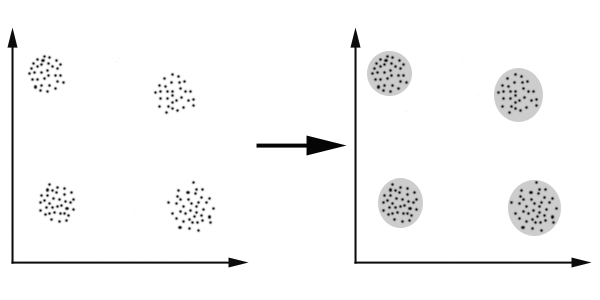
\includegraphics[height=1.5in, width=4in]{clustering}
    \caption{The result of appplying a clustering algorithm to unlabeled data. Four distinct clusters have been detected.}
    \label{ClusteringExample}
  \end{center}
\end{figure} 

\subsection{Vector space representation}

Document need to be preprocessed in order to be in a form that will allow us to perform clustering. 
The most common approach is to use the vector space representation model. The vector space representation transforms the 
documents into vectors of term frequencies which can then be used as a means to assess the similarity between documents.\\
We can represent each document in a dataset by a vector of identifiers. Usually, these identifiers are the distinct words in the document and 
the resulting vector is called term-frequency vector. If we combine all the vectors for the documents in our dataset we will end up with an 
\boldmath $m \times n$  \unboldmath  matrix \boldmath $A$ \unboldmath. Each of the $m$ documents in the document collection are assigned a row 
in the matrix, while each of the $n$ unique terms in each document are assigned a column in the matrix. A non-zero element $a_{ij}$ in \boldmath 
$A$ \unboldmath, indicates not only that term $j$ occurs in document $i$, but also the number of times the term appears in that document. Since the number of terms in a given 
document is typically far less than the number of terms in the entire document collection, A is usually very sparse.\\
For example in Table 3.1 we see that $Document1$ contains three instances of the word team, while football occurs five times. We can also infer that
the words ball and world are missing for the entire document, as indicated by the value of zero at those entries of the matrix.\\  
The main advantage of transforming the documents in the vector space is that we can define vector-space similarities between documents and therefore
we can apply clustering algorithms on the document collection. In section we provide a more detailed discussion on similarity metrics and the vector space 
representation is used in clustering documents.

\begin{table}[tbp]
\centering
\begin{tabular}{ l  l  l  l  l  l  l }
  \hline
  \textbf{Document} & \textbf{team} & \textbf{ball} & \textbf{football} & \textbf{countries} & \textbf{world} & \textbf{england} \\ \hline
  \emph{Document1} & 3 & 0 & 5 & 1 & 3 & 1 \\
  \emph{Document2} & 2 & 1 & 2 & 0 & 8 & 2\\
  \emph{Document3} & 1 & 5 & 3 & 0 & 1 & 3\\
  \emph{Document4} & 5 & 0 & 1 & 2 & 5 & 4\\
  \hline
\end{tabular}
\caption{Term-frequency vector representation of documents}
\label{termfrequencyTable}
\end{table}

\subsection{Assigning weights to terms with TF-IDF weighting}
Once a document is transformed in its term-frequency vector we can assign weights to each term in the vector. So far the term-frequency vectors treat 
all the terms as equal but this may not be the case. For example, a word that appears more frequently than others in a document could be considered as an 
important word. At the same time words that appear frequently in the corpus, such as 'a', 'the', 'and', are not very useful and their 
importance must be discounted. \\
The most common method to solve this problem is the TF-IDF weight (TF-IDF stands for term frequency-inverse document frequency) which quantifies the importance of a term in a document of a document collection. More specifically, the more a word occurs in a document, and the less it occurs in the rest of the coprus, the higher its TF-IDF weighting 
will be. Mathematically, TF-IDF is expressed as:\\
\begin{eqnarray}
tf-idf_{t,d} = tf_{t, d} \times idf_t
\end{eqnarray}

where $tf_{t, d}$ is the importance of term $t$ in document $d$ and $idf_t$ is the importance of term $t$ relative to the entire corpus. $tf_{t,d}$ is higher when the term occurs many times in the document and $idf_t$ is higher when it occurs rarely in the dataset. Therefore, the TF-IDF weighting for a term is very high if the term occurs frequently in a single document but very rarely in the entire corpus and it is low when the term either occurs rarely in a document or frequently in the entire corpus. TF-IDF is widely used to compare the similarity between documents and a common use case is for search queries where the similarity of a query $q$ with a document $d$ is calculated using TF-IDF, providing
a sorted list of the most relevant documents. 
\\
   
\subsection{Feature selection}
TODO: Discusss feature selection methods used in our system.

\subsection{Distance measures}
In data mining applications including clustering we must decide whether two objects are similar or dissimilar. In document clustering we wish to 
assess how similar are two documents in comparison to one another. Based on the similarity between two objects we can make the decision whether to
group them in the same cluster or not. In this section we present three commonly used similarity measures which will be used throughout our work. 

\subsubsection{Euclidean distance}
Euclidean distance is probably the most popular distance measure and can be thought as the straight line connecting the two data points that we try to compare.
Let the two data points be $i = (x_{i,1}, x_{i,2},...,x_{i,p})$ and $j = (x_{j,1}, x_{j,2},...,x_{j,p})$ where $p$ is the number of the numeric attributes. The Euclidean distance between $i$ and $j$ can then be defined as:\\
\begin{eqnarray}
d(i,j) = \sqrt{(x_{i,1} - x_{j,1})^2 + (x_{i,2} - x_{j,2})^2 + ... +(x_{i,p} - x_{j,p})^2 }
\end{eqnarray} 

Euclidean distance is the default distance measure used with the k-Means algorithm. 

\subsubsection{Cosine similarity}
The similarity of two documents which are represented as term vectors, corresponds to the correlation between the vectors. This is calculated as the cosine of the
angle between vectors, the so-called cosine similarity. Cosine similarity is widely used for text documents and especially in clustering documents. Let $x$ and $y$ be 
two vectors for comparison. Cosine similarity is defined as:

\begin{eqnarray}
sim(x,y) = \frac{x \cdot y }{\norm{x} \norm{y}} 
\end{eqnarray} 

where $\norm{a}$ is the Euclidean norm of vector $a$. This measure computes the cosine of the angle between the vectors x and y with a cosine value of $0$ meaning that the two vectors are at 90 degrees to each otther and therefore are not a match. If the cosine value is $1$ then the two vectors are identical and they are a perfect match. 

\subsubsection{Jaccard coefficient}
The Jaccard coefficient measures similarity as the intersection divided by the union of the objects. For text document, the Jaccard coefficient compares the sum weight of shared terms to the sum weight of terms that are present in either of the two document but are not the shared terms.

\begin{eqnarray}
sim(i,j) = \frac{q}{q + r + s}  
\end{eqnarray} 
where $q$ is the number of variables that are positive for both objects, $r$ is the number of variables that positive for $i$ and negative for $j$ and $s$ is the  number of variables that are positive for the $j$ and negative for $i$.


\subsection{Clustering methods}
There are many clustering algorithms and usually the belong to one of the following categories, as they are described in [put reference to the book]:

\begin{itemize}
 \item \textbf{Partitioning methods:} Partiotioning methods operate on a number of data points and form partitions of the data where each partition is a cluster. Usually, these methods have the restriction that each object must belong to a single cluster. They are only effective for a small to medium datasets. 
 \item \textbf{Hierarchical methods:} A hierarchical method creates a hierarchical decomposition of the given set of data objects. These methods can be firther subdivided 
 in agglomerative and divisive, based on how the decomposition is formed. Hierarchical methods suffer from the fact that erroneous merges or split cannot be undone. 
 \item \textbf{Density-based methods:} These methods, unlike most other techniques, can find clusters of arbitrary shapes. They can do so by employing the notion of density. The
 main idea is to keep growing a cluster as long as the density of a 'neighborhood' exceeds some threshold. Therefore, clusters are dense regions of data points that are separated 
 by low-density regions.
 \item \textbf{Grid-based methods:} Grid-based methods quantize the space into a number of cells which form a grid structure, All the clustering operations are performed on the grid structure. Since the provessing time is only dependent on the number of cells and not the number of data points these methods have fast processing time. 
\end{itemize}\vspace{15pt}

Below we outline the basic clustering methods that will be used in our system and we look into their key ideas that will guide 
our implementation. 

\subsubsection{k-Means algorithm}
k-Means algorithm belongs to the partioning methods category. A partitioning method distributes the objects in $D$  into k clusters, $C_1, ..., C_k$, such that $C_i \subset D$ and $C_i \cap C_j = \emptyset$ for $(1 \leq i, j \leq k)$. k-Means is a centroid-based technique whic means that a cluster, $C_i$, is represented by a centroid which can be the mean of all the points in the cluster. Practically, this representation is the centre point of the cluster. \\
More specifically, the k-Means algorithm starts by randomly selecting k of the object in D, and each one represents a cluster centre. Then for each of the remaining objects in D, the algorithm calculates the distance between each of the k cluster centres. The closest cluster is selected and that point is assigned to this cluster. The mean of each cluster is re-calculated after a new point has been assigned to it. At this point the k-Means algorithm iteratively tries to improve the within cluster variation (improving an objective function) by reassigning all the objects according to the new cluster centres. The algorithm continues until it converges to the point where the clusters formed in the previous iteration are the same to the clusters formed in this iteration. Figure 3.4 (TODO:Put image ref) depicts a simple example of the k-Means algorithm with two clusters. In the first image, the two centroids, which are depicted as dark circles are initialised to a random position in the space. In the second image each of the data points is assigned to the nearest centroid and in this case A and B are assigned to the top centroid and C, D, and E are assigned to the bottom centroid. In the third image, each centroid's average is re-calculated and moved to its new position. When the assignments are calculated again, it turns out that C is now closer to the top centroid, while D and E remain closest to the bottom one. Thus, the final result is that A, B, and C belong in one cluster, and D and E in the other. \\

\begin{figure}[!htbp]
  \begin{center}
    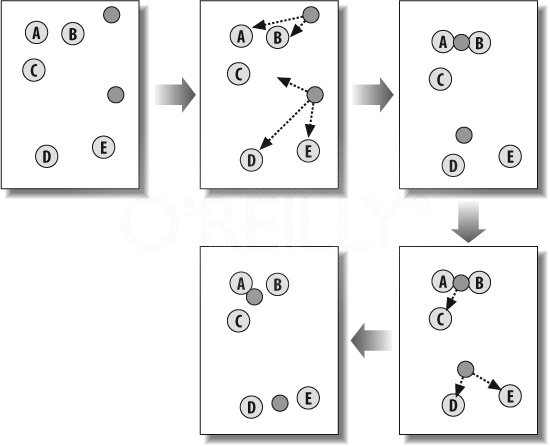
\includegraphics[height=2.5in, width=4in]{kmeans-example}
    \caption{k-Means clustering with two clusters}
    \label{kMeansExample}
  \end{center}
\end{figure} 
 
The algorithm is not guaranteed to converge to a global optimum and the results depend on the initial allocations of the k centres. The time complexity is $O(nkt)$ where n is the total number of of objects, k is the number of clusters and t is the number of iterations. Therefore, the k-Means algorith is relatively scalable. 

\subsubsection{DBSCAN algorithm}
k-Means algorithm and hierarchical clustering algorithms are very good at clustering spherical-shaped clusters. However, they are not able to detect clusters of arbitrary shape such as the one below.  \

\begin{figure}[!htbp]
  \begin{center}
    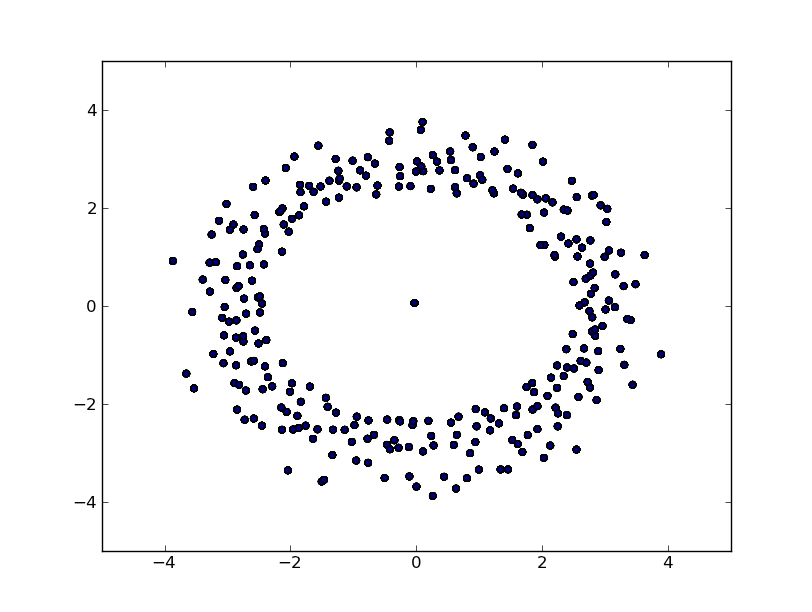
\includegraphics[height=3in, width=4in]{dbscan-example}
    \caption{The DBSCAN algorithm belongs to the density-based methods which can find clusters of arbitrary shapes (not only spherical).}
    \label{DBSCANExample}
  \end{center}
\end{figure} 

In order to alleviate the problem one have to look into density-based clustering algorithms. These algorithms model clusters as dense regions in the data space. One of the most popular algorithms of this kind is the Density-Based Clustering Based on Connected Regions with High Density (DBSCAN). \\ 
DBSCAN defines density of an object $o$ as the number of objects close to $o$. DBSCAN finds core objects which are objects with dense neighborhoods. Then it connects those core objects and their neighborhoods to form clusters. In order to assess density, DBSCAN uses a constant $\epsilon  > 0$ which defines the radius of the neighborhood of an object $o$ and then finds the number of objects in the neighborhood. If the number is above a threshold $MinPts$ then the neighborhood is considered dense. Given a set, $D$, of objects, we can identify the core objects using $\epsilon$ and $MinPts$. The problem of clustering then reduces to the task of finding dense regions using the core objects and their neighborhoods. \\\\
The complexity of the algorithm in our implementation is $O(n^2)$ but it can be reduced to $O(n\log n)$ if a spatial index is used. This means that this algorithm doesn't allow us to scale it up to large volume of data. The main disadvantage of the DBSCAN algorithm is that the user has to pass the $\epsilon $ and the $MinPts$ parameters which usually is a difficult task and some datasets are very sensitive to variations of these parameters. 

\subsubsection{Non-negative matrix factorisation algorithm}
Non-negative matrix factorization (NMF) is not a clustering algorithm per se but it can be shown that it is equivalent to a relaxed form of k-Means algorithm. This algorithm takes as input the term-document matrix, constructed during clustering pre-processing and decomposes it into two other matrices. The first one is a feature-term matrix (or features matrix) and the other a document-feature matrix (or weight matrix). In the latent semantic space derived by the NMF, each axis captures the base topic of a particular document cluster, and each document is represented as an additive combination of the base topics. The cluster membership of each document can be easily determined by finding the base topic (the axis) with which the document has the largest projection value. The only constraint of the algorithm is that the two derived matrices should be non-negative.\\\\ 
In the context of document clustering we use matrix factorisation to reduce a large set of documents to a smaller set that captures their common topics (features) [put ref to the book Collective Intelligence ]. We start with a term-frequency matrix and we wish to factorise this matrix to get the two matrices we mentioned above. The features matrix has a row for each feature and a column for each term (word). An example of such a matrix is shown below. The values indicate how important a word is to a feature. Each feature represents a topic that is implied from a set of documents. 

\[
\bordermatrix{~ & football & ball & england & newspaper \cr
                  feature 1 & 1 & 0 & 3 & 2 \cr
                  feature 2 & 0 & 1 & 3 & 1\cr
                  feature 3 & 0 & 2 & 2 & 1\cr}
\]\\
The weights matrix maps the features to the documents. It has a row for each document and a column for each feature. The values indicate how much each feature matches to each document. An example of the weights matrix is shown below. 

\[
\bordermatrix{~ & feature 1 & feature 2 & feature 3\cr
                  Document 1 & 1 & 5 & 3\cr
                  Document 2 & 3 & 1 & 1\cr
                  Document 3 & 0 & 2 & 3\cr}
\] \\
The original matrix can be reconstructed by multiplying the weights matrix by the features matrix, although the resulting matrix would not be an exact reconstruction of the original one but an approximation. 

\subsubsection{Online clustering algorithm}
All the algorithms described above operate on the whole dataset, $D$, and sometimes this is not desirable or not even neccessary. Especially if the dataset is too large and we are concerned about performance and scalability. Therefore, a family of algorithms have been studied in order to modify common algorithms for scalability. These algorithms are called sequential or online clustering algorithms. By online in this context we mean an algorithm that does not keep all the data objects in memory at the same time, but processes them sequentially, keeping only a subset if them.\\
Suppose we are given a sequence of N tweets $T = {t_1, ..., t_N}$ where each $t_i$ is a vector of $a$ attribute values, and we want to split them into $K$ clusters. Each cluster is described by a prototype vector $p_i = {p_1, ..., p_f}$ where $i = 1, ..., K$. Given that the task of finding good clusters is to minimize an objective distance function $J$ the algorithm works as follows:
\begin{enumerate}
   \item Pick the next example in the sequence T
   \item Compute the distances from this example to all the cluster prototypes and pick the minimum one.
   \item Update the prototype vector in order to come closer to the current example  
   \item Goto step 1  
 \end{enumerate} 
 
The implementation of our online algorithm is based on the work proposed in the paper "Improving the Robustness of ‘Online Agglomerative Clustering Method’ Based on Kernel-Induce Distance Measures" by Zhang et al. They have used kernel-functions for distance measures and post-processing filtering is performed to remove noise from data. Extending their work, in our implementation we have tried to increase its scalability by allowing only a sliding window of $n$ tweets to be in memory each time when the term-document vectors are calculated. 

\section{Automatic text summaries}\label{SummaryGen}

Another integral component of our framework is the module repsonsible for generating automatic summaries of the events. In Chapter \ref{chap:Introduction}
we described the problem of event summarisation as the task that will extract the top tweets for an event that are most helpful for a human to understand the event.
The term 'helpful' is vague and therefore we have defined three criteria, described in [TODO: put ref for the paper Selecting Quality Twitter Content for Events ] that will evaluate qualitatively our summaries and guide our implementation choices. The three criteria are:

\begin{itemize}
 \item \textbf{Quality:} It refers to the textual quality of the messages, which reflects how well they can be understood by a human.
 \item \textbf{Relevance:} It refers to how well a Twitter message reflects information related to its associated event.
 \item \textbf{Usefulness:} It refers to the potential value of a document for someone who is interested in learning more about an event.
\end{itemize}\vspace{15pt}

\subsection{Generating automatic document cluster summaries}
In general, in automatic text summarisation we are interested in generating a shortened version of a large corpus or document but maintaining the integrity and meaning of 
the original text. There are to variations of the automatic text summarisation: the extractive summarisation method which produces summaries by choosing a subset of the sentences
in the original document or documents and abstractive summarisation, where the information in the text is rephrased.\\\\
In our case the task is to reduce a large set of tweets in a smaller subset by ranking the individual tweets in a subset and selecting the top ranking ones.
In our project we consider two methods extractive summarisation methods, the centroid-based summarisation and the LexRank algorithm.

\subsubsection{Centroid-based summarisation}
The centroid similarity approach computes the similarity of each message to its associated event cluster centroid. The cluster centroid is calculated by averaging the weight across all the document TF-IDF weigthed term-frequency vectors in a specific event. The method then selects the documents with the highest similarity value. The implicit assumption is that a cluster’s centroid emphasises important terms which are relevant to the event. For example a cluster describing the topic of some protesters giving flowers to policemen in Cairo would give higher weight to the terms "protesters", "flowers" and "policemen". Therefore documents with high similarity to these key terms are more likely to reveal key aspects of the event which is highly desired by the relevance and usefulness goals. Additionally, the quality criterion is satisfied since the centroid weights are based on frequency across all messages, and therefore they contain no typos or spelling mistakes (which can greatly affect the quality of a document). 

\subsection{LexRank algorithm}
[TODO explain LexRank]

\subsection{Detecting named entities and locations in documents}
The summaries produced by the algorithms described above are a good representation of the event and can help a human to understand the event. However, sometimes some additional
information is needed to comprehend an event. In Chapter \ref{chap:Introduction} we described an event as a collection of attributes such as keywords, geographic location and entities involved. Therefore, we wish to be able to automatically extract these attributes for an event and included them in the summary of an event. The keywords describing the event are simply the words having the highests weight in an event cluster and can extracted very easily. For the named entities and locations we have to use a technique called named entity extraction which is part of the NLP algorithms. The method takes as input a piece of text and locates and classifies atomic elements in text into diffeent categories such as the names of persons, organisations and locations.


\section{Twitter user classification}
Different types of users interact and disseminate information daily on Twitter. Depending on the type of user we expect the content of a tweet to vary and consequently the quality of a tweet will vary too. For example renowned journalists are more likely to produce high quality tweets which easily be trusted as a reliable source of information. On the other hand tweets generated by a tweet bot might be considered unreliable since bots are known to release rumors. Therefore, it is crucial to be able to distinguish different types of users in order to ensure that we will extract high quality events that provide useful information and not just rumors. Additionally, it is interesting in its own right to investigate what is the distribution of the users tweeting for an event. For example, we would like to find out whether activists can start and sustain an event discussion online or whether celebrities or political figures can spark the interest of other Twitter users. In order to do that we need to find a way to classify users.\\\\ 
Classification is the process of finding a model that describes and classifies data classes. The model is derived based on a set of training data (data objects which their class labels are known). Then the derived model is used to predict the class of an uknown instance which is presented to the learning system.    

\subsection{Decision trees}
Decision Tree learning is a method for approximating discrete classiffication functions using a tree-based representation. We can make use of this method to inductively infer [put ref here] unknown relations within our dataset. A nice property of the decision trees is that they can also be represented as a set of if-then rules, therefore the task of interpreting them is an easy task for a human. A learned decision tree is able to classify a new instance by sorting it down the tree to the appropriate leaf node, then returning the classification associated with this leaf. Every node in the tree tests some attribute value of each new instance, and the branches of each node represent a possible value for that attribute.\\\\
Figure 3.6 illustrates a simple decision tree, which classifies a day's weather conditions according to wether they are suitable for playing tennis [put ref to mitchell's book]. If the decision tree is presented with an example of a day when the outlook is sunny, the temperature is hot, the humidity is high and the wind is strong then this example would be sorted down the leftmost branch and therefore would be classified as negative, i.e, this day is not suitable for playing tennis. Alternatively, the tree could be represented as if-then rules:\\  


\begin{center}
  (Outlook = Sunny $\wedge$ Humidity = Normal)\\
  $\vee$ (Outlook = Overcast)\\
  $\vee$ (Outlook = Rain $\wedge$ Wind = Weak)
\end{center}

\begin{figure}[!htbp]
  \begin{center}
    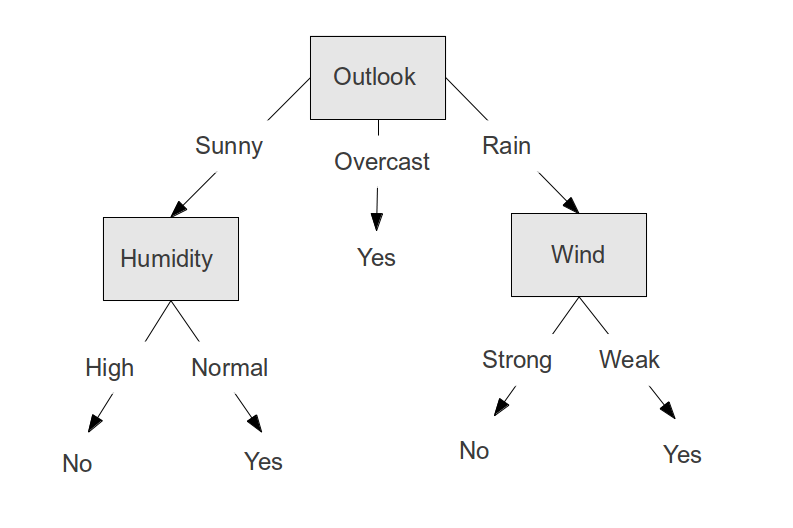
\includegraphics[height=2in, width=4in]{decision-tree-example}
    \caption{A simple decision tree.}
    \label{DecisionTreeExample}
  \end{center}
\end{figure} 

\subsection{Neural networks}
[TODO explain Neural Nets]

\section{Summary}

Show a simple diagram with a lot of tweets becoming vectors and then those becoming clusters and then some of them events.
This is the outout of the algorithm.

% ------------------------------------------------------------------------

%%% Local Variables: 
%%% mode: latex
%%% TeX-master: "../thesis"
%%% End: 

\chapter{Design and implementation of the event detection and summarisation methodology}\label{DesignAndImplementation}
\ifpdf
    \graphicspath{{Chapter3/Chapter3Figs/PNG/}{Chapter3/Chapter3Figs/PDF/}{Chapter3/Chapter3Figs/}}
\else
    \graphicspath{{Chapter3/Chapter3Figs/EPS/}{Chapter3/Chapter3Figs/}}
\fi

The aim of this chapter is to give a thorough description of the implementation of our methodology for event detection and summarisation. The theoretical concepts introduced in Chapter \ref{TheoreticalFramework} are now the building blocks of this methodology. Each of these building blocks can be used in isolation but when we combined these individual components the end product is a data mining toolset which is able to detect and summarise events. We list and provide an explanation of the individual components of this toolset and also explain our reasoning for certain design choices. 

\section{System Overview}
Figure \ref{SystemOverview} shows an overview of the system architecture which is a pipeline of the individual components we described
in Chapter \ref{TheoreticalFramework}. Each one of these components is depicted as an independent module in the figure.  
Initially, historical tweets from a service provider (Twitter API or another provider) are retrieved and stored in an 
appropriate format in the database. Subsequently, the system receives a stream of tweets from the database and processes and 
transforms them in a format that is appropriate for clustering. The next step in the pipeline is the actual clustering of the tweets 
in order to detect groups of tweets discussing the same topic. Then, the extracted clusters are processed in order to identify the events 
and generate their summaries. Finally, a visual representation of the results should be generated in order to aid understanding of the events.\\

\begin{figure}[htbp]
  \begin{center}
    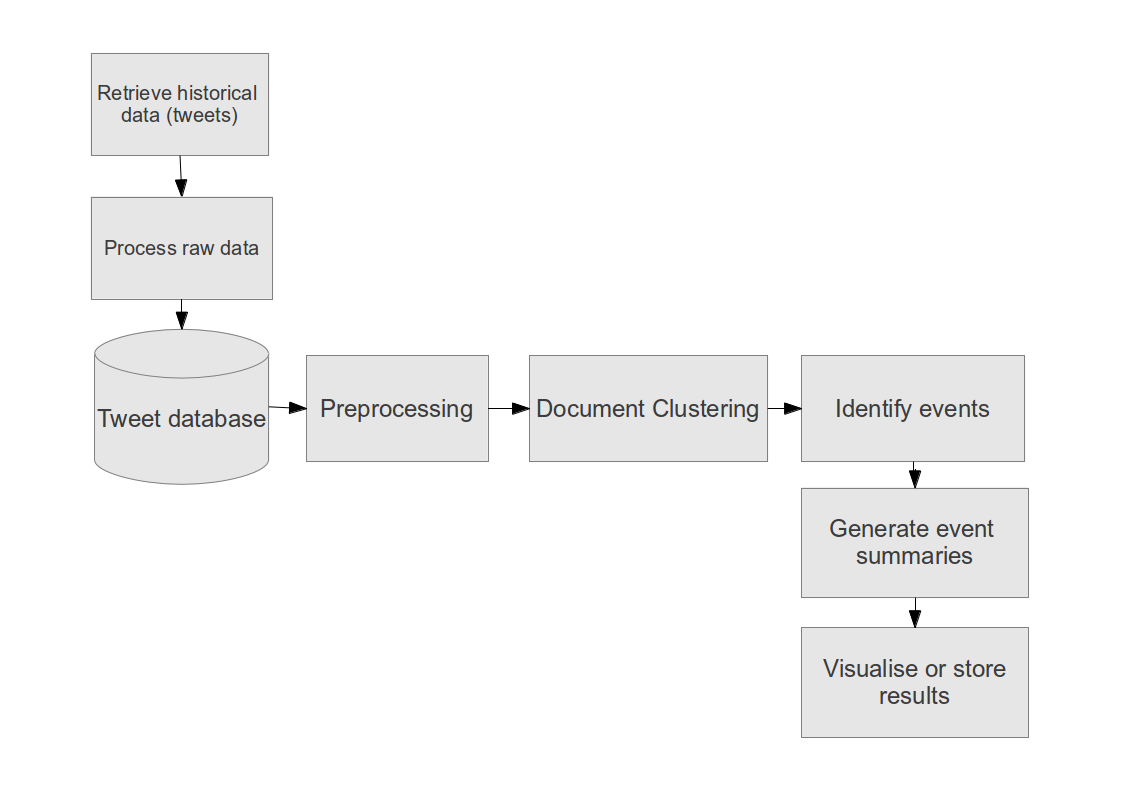
\includegraphics[height=3in, width=6in]{system-overview}
    \caption{System overview - The event extraction system comprises of several independent components.}
    \label{SystemOverview}
  \end{center}
\end{figure}

\subsection{Tools}
In the process of implementing the system we have mainly used our implementation of the algorithms but several third-party 
software libraries were used to implement the subcomponents of the system. Here we describe the main tools we have used.\\ 

\begin{itemize}
 \item \textbf{Python\footnote{http://docs.python.org/tutorial/}:} Python is a powerful programming language with efficient high-level data structures. We have selected Python due to its wide range of third-party libraries which can be used for mathematical operations. Additionally, is an ideal language for scripting and rapid application development which is desired in our project since we wanted to test our implementation as quickly as possible.  
 \item \textbf{Natural Language Toolkit\footnote{http://nltk.org/} (NLTK):} NLTK is a complete platform for building Python programs to work with human generated text content. It provides built-in methods for text tokenisation and sentence segmentation as well as modules for named-entity recognition.    
 \item \textbf{Lucene\footnote{http://lucene.apache.org/core/}:} Lucene is a high-performance, full-featured text search engine library written entirely in Java. Lucene allows us to build search engines or any other application that requires full-text search. In our case we use Lucene to build our inverted index structure. More specifically, we use PyLucene which is a library with Python wrappers for Lucene's functions.
 \item \textbf{Orange\footnote{http://orange.biolab.si/}:} Orange is an open-source data mining library. It contains a wide range of methods to perform several data mining and machine learning methods such as classification and clustering.    
 \item \textbf{Numpy\footnote{http://numpy.scipy.org/}:} NumPy is a Python library which is concerned with adding support for large, multi-dimensional arrays and matrices. It is used throughout our implementation to perform all the matrix and vector operations.
\end{itemize}\vspace{15pt}

\section{Data Retrieval}
A vital part of our system is the retrieval of a large amount of historical tweets. The first obvious choice is the Twitter API which provides tweets, user profiles and several metadata related to Twitter. They also provide a streaming API which is commonly used to collect tweets in real time. However, the main problem with the Twitter API is that it has a very restrictive limit policy (150 requests per hour) and it does not provide access to tweets posted more than a few days ago. This raises a significant barrier for our project since we require access to historical data. The solution is to use other archiving services and there are numerous possibilities. Additionally, it is essential for us to have direct access to their database through an API and unfortunately, most of them do not provide an API. We have found that Topsy \footnote{http://topsy.com/} provides an excellent API \footnote{http://code.google.com/p/otterapi/} and direct access to tweets covering a period from 2009 up to the present day. Additionally, Topsy API is free and the limit policy allows us to retrieve our data easily. Therefore, we have decided to use Topsy Otter API with its Python bindings.

\section{Raw text processing}
The raw tweets received from Topsy are not processed yet and therefore we must apply some preprocessing steps before storing them in the database. The reasons for pre-processing were outlined clearly in section \ref{RawDataProcessing}. Figure \ref{RawTextProcessingOverview} depicts the subcomponents of the raw text preprocessing module.\\\\

\begin{figure}[htbp]
  \begin{center}
    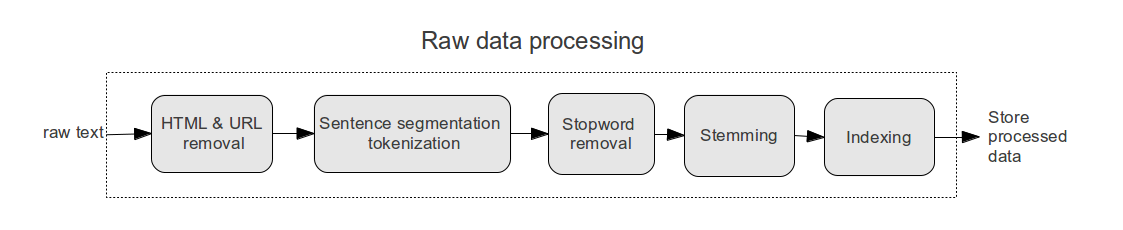
\includegraphics[height=1.5in, width=6in]{raw-data-processing}
    \caption{The raw data processing module - All the steps neccessary to convert raw documents to a format suitable for storage in a database.}
    \label{RawTextProcessingOverview}
  \end{center}
\end{figure} 
\noindent \textbf{HTML and URL removal:} Firstly, we need to remove the URLs and HTML tags from the tweets since they are useless for clustering. In order to do so we have used regular expressions which capture any possible format of URLs or HTML code.\\\\
\textbf{Sentence segmentation and tokenisation:} For the implementation of this module we have used the default sentence segmenter of NLTK and the WordPunctTokenizer to tokenise the resulting sentences. The reason behind the choice of the WordPunctTokenizer is due to the fact that it can handle alphabetic and non-alphabetic characters. Since it is common to use non-alphabetic characters in a tweet, this tokeniser made it easy to remove characters such as '.' and ','. Consider for example the following tweet:
 
\begin{figure}[htbp]
  \begin{center}
    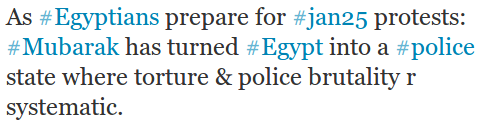
\includegraphics[height=1in, width=4in]{tweet-text}
    \label{TweetText}
  \end{center}
\end{figure}

\noindent The output from this module will be a list of words containing the terms \textbf{[ 'as', 'egyptians', 'prepare', 'for' 'jan25', 'protests', 'mumbarak', 'has', 'turned', 'egypt', 'into', 'a', 'police', 'state', 'where', 'torture', 'police', 'brutality', 'r', 'systematic' ]}. Note that characters '.', '\#', '\&' and ':' have been removed. \\

\noindent \textbf{Stopword removal:} The next step is to remove common English words that do not provide any information. NLTK provides a dictionary of the English stopwords and we have used it to filter out stopwords from the tweets. Using the list of words extracted for the example above the output of the stopword removal module will be: \textbf{['egyptians', 'prepare', 'jan25', 'protests', 'mumbarak', 'turned', 'egypt', 'police', 'state', 'torture', 'police', 'brutality', 'r', 'systematic' ]}

\noindent \textbf{Stemming:} Once we have the list of our terms we can use a stemming algorithm to reduce the words to their root. Our implementation uses the widely used Porter stemmer which is also implemented in NLTK. The final list of words after the stemming becomes \textbf{['egyptian', 'prepar', 'jan25', 'protest', 'mumbarak', 'turn', 'egypt', 'polic', 'state', 'tortur', 'polic', 'brutal', 'r', 'systemat' ]}\\

\noindent \textbf{Indexing:} Just before storing the tweets in the database, we take a last step which is to index the tweets. For each word occurring in our corpus we aggregate all the tweets, that contain that term, and the position of that word in the document. Effectively, we create a mapping from a word to a list of documents. In our implementation the inverted index is very important since it allows us to construct term-frequency vectors easily and filter terms and documents. For example, using our index we can find the words that appear either too often or less frequently and filter them out. This is used to reduce the dimensionality of our dataset by removing unnecesary words. Alternatively, we
can remove documents/tweets which contain keywords that appear too often or less frequently. In our implementation we have used PyLucene which is the Python equivalent of the Lucene indexing library. The library allow us to do what we have discussed above and in addition it provides helper functions such as the calculation of the TF-IDF weightings for a dataset.
 
\section{Clustering}
So far we have managed to retrieve and store historical tweets in our database. The next module in our pipeline is to perform clustering on the tweets and identify clusters which discuss the same topic. The clustering module (Figure \ref{ClusteringOverview}) must construct the term-frequency vectors by processing the dataset and subsequently to apply a clustering algorithm on the dataset. 

\begin{figure}[htbp]
  \begin{center}
    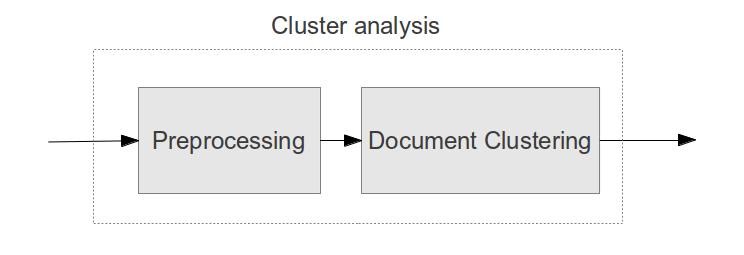
\includegraphics[height=1.5in, width=4in]{clustering-overview}
    \caption{The cluster analysis module - The dataset is processed to construct the term-frequency vectors and then a clustering algorithm is used to identify the clusters.}
    \label{ClusteringOverview}
  \end{center}
\end{figure} 

\noindent There are several candidates algorithms for clustering documents and we have decided to implement four of them. The theoretical background of these algorithms is outlined in Chapter \ref{TheoreticalFramework} and in Chapter \ref{Evaluation} we present a thorough comparison of these algorithms with respect to their performance in clustering tweets.  
In the next section we provide our implementation of these algorithms and the components that are needed for clustering. All the clustering and summarisation algorithms were implemented by us using the help of the aforementioned third-party tools.  

\subsection{Software implementation}
The four different algorithms presented in this section are the k-Means, DBSCAN, Non-negative Matrix Factorisation (NMF) and online clusterers. Although these methods are fundamentally different they share some common functionality. For example the preprocessing steps, such as the construction of the term-frequency vectors is identical for all of them. Also, all of the algorithms output the clusters using the same format and therefore the methods for visualising the clusters will be identical. The architecture of the software components responsible for implementing the clustering functionality tries to incorporate this common functionality as well as accomodating the different core implementation of each algorithm. The UML diagram (Figure \ref{UMLClusterers}) below illustrates the different components of the clustering module. The AbstractClusterer class implements all the common functionalities such as add\_document, construct\_term\_freq\_matrix, plot\_scatter and dump\_clusters\_to\_file. Since each algorithm uses a different method to perform the actual clustering task, the AbstractClusterer class does not provide any implementation for the "run" function. This is the responsibility of each derived clusterer. The use of an AbstractClusterer makes our design extremely modular and reusable since we can switch different implementations at any time with minimal changes in the code.

\begin{figure}[htbp]
  \begin{center}
    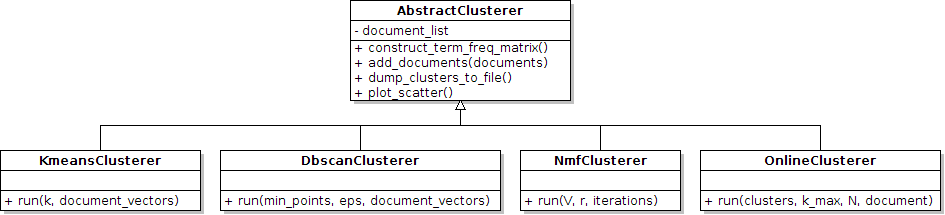
\includegraphics[height=2.0in, width=6in]{clusterers-uml}
    \caption{The four derived clusterers share common functionality which is implemented in the AbstractClusterer class. }
    \label{UMLClusterers}
  \end{center}
\end{figure}    

\subsubsection{AbstractClusterer}
\noindent The main functionality of the AbstractClusterer is to construct the term-frequency vector for each document and consequently the term-frequency matrix $a$ which has a row for each document and a column for each distinct term in the dataset. This will convert the corpus in the vector space representation. Listing \ref{AbstractClustererSnippet} shows the pseudocode for implementing the construct\_term\_freq\_matrix() function. It retrieves the dataset from the database and finds all the distinct terms that occur across all the documents. Then the term-frequency matrix is initialised and we iterate over the documents filling in the elements of the matrix with the TF-IDF weight of each term. The function returns the matrix $a$.

\begin{lstlisting}[language=Python, label=AbstractClustererSnippet, caption=Pseudocode for constructing the term-frequency matrix for a dataset]
def construct_term_freq_matrix(corpus):
  '''
  Inputs: 
  corpus: The collections of documents we will cluster
  
  Outputs:
  a: A nxm matrix where n is the number of documents 
     in the corpus and m the number of distinct terms
     in the corpus.  
  '''
  terms = find_distinct_terms(corpus)
  a = initialise_term_frequency_matrix(rows=len(corpus), 
                                        columns=len(terms))
  
  for i, document in enumerate(corpus):
    for term in document
      a[i][term] = tf_idf(term, document, corpus)
    
  return a 
\end{lstlisting}

\noindent In the next pages we discuss the implementation of the concrete clusterers which implement the second subcomponent of the cluster analysis module.

\subsubsection{k-Means clusterer implementation}
Listing \ref{KmeansClustererSnippet} shows the pseudocode for k-Means clustering algorithm. The algorithm works by randomly initialising k centroids and then finding out which document vectors are closest to the centroid. Then the centroid is recomputed based on the mean of the vectors belonging to this centroid and this mean value becomes the new centroid. An additional check is performed again to ensure that all the vectors are still belonging to that cluster after the recomputation of the centroid. This procedure is repeated until there are previous cluster membership has not changed. Note that the distance() function can be any of the three distance measures described in the previous chapter.

\begin{lstlisting}[language=Python, label=KmeansClustererSnippet, caption=Pseudocode for k-Means algorithm]
def run(k, document_vectors):
  '''
  Inputs: 
  k: the number of clusters
  document_vectots: the set of n document 
                     vectors I={i1,i2,..,in}
  
  Outputs:
  C: cluster centroids {c1, c2, ..., ck}
  m: I --> C the cluster membership
  '''
  C = random_centroid_initialisation()
  
  distances = []
  for vector in document_vectors
    for c in C:
      dist = distance(c, vector)
      distances.append(dist)
    m[vector] = min(distances)

  while has_changed(m):
    for c in C:
      c = recompute_centroid(c, vectors_of(c))   
    
    for vector in document_vectors
      for c in C:
        dist = distance(c, vector)  
        distances.append(dist)
      m[vector] = min(distances)
  return C, m

\end{lstlisting}
\subsubsection{DBSCAN clusterer implementation}
Listing \ref{DbscanClustererSnippet} shows the pseudocode for the DBSCAN clustering algorithm. Initially,
all documents are marked as unvisited and the cluster list is empty. Then the algorithm randomly selects a new document vector, marks it as visited and finds all its neighbours than are within a distance $eps$. The set of neighbours is called $\epsilon$-neighbourhood and we denote it here by N. In order to calculate the distance we use one of the three predefined distance measures. If N does not contain at least min\_pts then we mark this vector as a noise point. Otherwise, a new cluster is created which contains this vector and all the objects in N are added to a candidate set. DBSCAN iteratively adds to the new cluster those documents in the N that do not belong to any cluster. For any object in the $\epsilon$-neighbourhood DBSCAN checks again its own $\epsilon$-neighbourhood N' and if it has at least min\_pts those document vectors are added to the N. This continues, with DBSCAN adding new documents in the new cluster, until N is empty. Finally, to find the next cluster DBSCAN selects a new unvisited document vector and continues the same process until all vectors have been visited.  

\begin{lstlisting}[language=Python, label=DbscanClustererSnippet, caption=Pseudocode for DBSCAN algorithm]
def run(min_points, eps, document_vectors):
  '''
  Inputs: 
  eps: the radius parameter
  min_pts: the neighbourhood density threshold.
  document_vectors: the set of n document vectors 
                     I={i1,i2,..,in}
  
  Outputs:
  C: the clusters and the document vectors 
     belonging to them
  '''
  C = [] #The cluster list
  mark_all_vectors_as_unvisited(document_vectors)
  
  while not all_is_visited(document_vectors):  
    vector = pick_random(document_vectors)
    mark_as_visited(vector)
    neighbours = get_neighbours(document_vectors, vector)
    if len(neighbours) >= eps:
      new_cluster = create_cluster(vector) 
      C.append(new_cluster)
      for n_vector in neighbours:
        if not is_visited(n_vector) 
          mark_as_visited(n_vector)
          n_neighbours=get_neighbours(document_vectors,n_vector)
          if len(n_neighbors) >= eps:
            neighbours.append(n_neighbours)
        if not_in_cluster(n_vector):
          new_cluster.add(n_vector)
    else:
      mark_as_noise(vector) 
  return C
\end{lstlisting}
\subsubsection{Non-negative matrix factorisation (NMF) clusterer implementation} Our NMF algorithm implementation is based on the paper \citep{lee99}. The method accepts as input the term-frequency matrix $V$ the number of basis vectors to generate $r$ and the number of optimisation iterations. The algorithm starts from non-negative initialisations for W and H and then iteratively updates W and H until a factorisation $V \approx WH$ such that $| V - WH |$ is minimal. If the number of maximum iterations has not been reached and the error did not change since the last iteration then the algorithm halts and return W and H. Listing \ref{NmfClustererSnippet} shows the pseudocode for the NMF algorithm. The notation $A.T$ indicates that we should take the transpose of the matrix $A$.
  
\begin{lstlisting}[language=Python, label=NmfClustererSnippet, caption=Pseudocode for the NMF algorithm]
def run(V, r, iterations):
  '''
  Inputs: 
  V: the matrix to factorize
  r: number of basis vectors to generate
  iterations: number of optimisation
             iterations to perform
  
  Outputs:
  W: a set of r basis vectors
  H: represenations of the columns of V in 
     the basis given by W
  '''
  
  C = size(V,1) #dimensionality of examples (# rows)
  N = size(V,2) #number of examples (columns)

  W = rand(N,r);
  H = rand(r,C);
  
  previous_error = 0
  error = 0
  for i in xrange(iterations):

    #Update W
    W2 = dot(dot(W, H), H.T) + 10**-9
    W *= dot(V[:,:], H.T)
    W /= W2
    
    #Update H
    H2 = dot(dot(W.T, W), H) + 10**-9
    H *= dot(W.T, V[:,:])
    H /= H2                                     
    
    previous_error = error
    error = sqrt( sum((V[:,:] - dot(W, H))**2 ))
    
    if i > 1 and error:
      if previous_error == error:
        break
  return W, H
  
\end{lstlisting}

\subsubsection{Online clusterer}
The previous algorithms operated on the dataset as a whole. Since we are interested in clustering a vast amount of documents these approaches are expensive. However, we can use a category of clustering algorithms called sequential or online clustering methods. The main difference is that they cluster each individual example sequentially by updating the clusters once this specific example is presented to the system. Therefore, an online algorithm is scalable. Usually, these kinds of algorithms are centroid-based and the mean values of centroids are updated using a moving average. This fact makes an online clusterer much faster than the other algorithms.\\\\
In our case, whenever we are presented with a new document the term-frequency vectors of all the previous documents must be updated. This operation is computationally expensive and we have implemented a simple refinement of this algorithm. Our version of the algorithm allows only a sliding window of $N$ tweets to be in memory each time the term-frequency vectors are calculated. For example if we are presented with the $ith$ document, denoted as $x_i$ and our window size is N then only the documents $\{ x_{i-1}, x_{i-2},..., x_{i-N}\}$ will be used for clustering. This can provide us with an extra performance boost but at the same time it decreases accuracy since we calculate our feature vectors on a limited number of documents.\\\\
Our implementation is illustrated in pseudocode in Listing \ref{OnlineClustererSnippet} and it can be summarised in three main steps: 

\begin{enumerate}
  \item Find the closest centroid and move it closer to the new document vector. 
  \item Merge the two closest centroids, c1 and c2, which means that we are left with a redundant centroid c2.
  \item Set the redundant centroid equal to the document vector. 
\end{enumerate}
These three steps satisfy three important criteria. Firstly, the within-cluster variance is minimised by Step 1 and the between-cluster distance is maximised by Step 2. Finally we capture the changes in the data distribution after a new document is clustered by Step 3 since we are treating each new document as an indication to a potential new cluster.\\\\
In the algorithm there are two cases when we need to update the location and the size of an existing centroid. The first one is when a centroid is the closest to a new document and it must be moved closer to it. The location of the closest centroid, $c$, is updated according to the following update rule location:
\begin{eqnarray}
c_{center} \leftarrow c_{center} + \frac{d_{center} - c_{center}}{c_{size} + 1}    
\end{eqnarray}  
where $c_{center}$ is the centroid's location, $c_{size}$ is the number of documents this centroid represents and $d_{center}$ is the document that we are trying to get closer to. The size of a centroid is increased by one each time a new document is assigned to it. The second case for updating is when two clusters, $c_1$ and $c_2$ need to be merged. The update rules for the location and the size are then defined as:
\begin{eqnarray}
c1_{center} \leftarrow \frac{c1_{center} \times c1_{size} + c2_{center} \times c2_{size}}{c1_{size} + c2_{size}} \\
\end{eqnarray}  
\begin{eqnarray}
c1_{size} \leftarrow c1_{size} + c2_{size} 
\end{eqnarray}  


\begin{lstlisting}[language=Python, label=OnlineClustererSnippet, caption=Pseudocode for the online clustering algorithm]
def run(clusters, k_max, N, document):
  '''
  Inputs:
  N: the size of the document window
  k_max: the maximum number of clusters we can identify 
  document: the new document to be clustered 

  Outputs:
  clusters: returns the updated clusters
  '''    
  #construct a new term-frequency vector based on the new
  #document and consider only the last N documents. 
  vector = construct_term_freq_vector(self.document_list, 
                                      document, 
                                      N)

  distances = []
  for centroid in clusters:
    dist = distance(centroid, vector)
    distances.append(dist)
  
  #find the closest centroid (Step 1)
  closest = min(distances)
  closest.add(vector)

  #update the centroids center  
  closest.size += 1
  closest.center += (vector-closest.center)/closest.size
  
  if len(clusters)>=k_max and len(clusters)>1:
    #merge the most similar clusters (Step 2)
    merged = merge_closest(clusters)
  
  
  #create a new cluster for this document (Step 3)
  newc = Cluster(vector)
  clusters.append(newc)
  return clusters
  
def merge_closest(clusters):
  c1, c2 = find_closest()
  c1.center=(c1.center*c1.size+
            c2.center*c2.size)/(c1.size+c2.size)
  c1.size+=c2.size
  c2.remove() #c2 is now merged with c1 so remove it
  return c1
    
\end{lstlisting}

\section{Identifying events}\label{IdentifyEvents}
[TODO: Complete this section]

\section{Generating automatic summaries}
So far we have managed to retrieve historical tweets from Twitter and identify clusters of topics that were discussed in them. After that we have filtered out the irrelevant clusters and kept the important ones which are considered as the events. Some of these events contain a lot of tweets and therefore it would be extremely tedious for a human observer to understand what happened during that event. Therefore, at this point we must implement our automatic summary generators. The main task here is to find the most important tweets, keywords and named entities. In the next sections we describe how we have implemented the functionality to extract this information. An overview of the summarisation module is shown in Figure \ref{SummarisationOverview}.  

\begin{figure}[!htbp]
  \begin{center}
    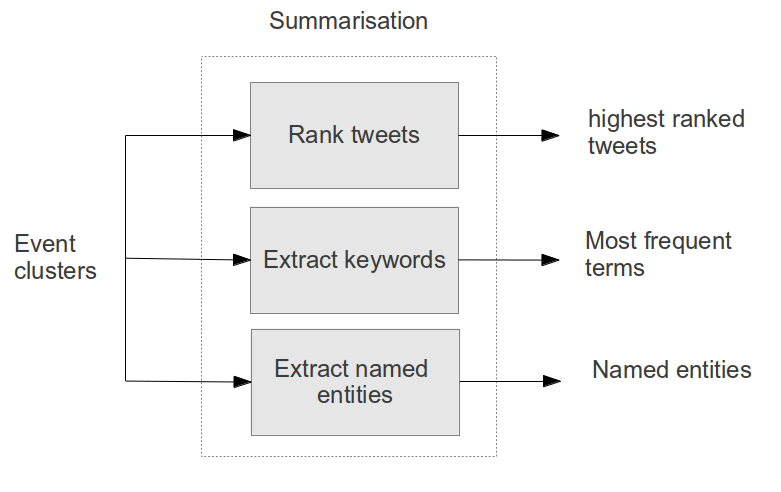
\includegraphics[height=3.0in, width=6in]{summarisation-overview}
    \caption{The summarisation module receives the event clusters and outputs the highest ranked tweetsm keywords and entities in each cluster.}
    \label{SummarisationOverview}
  \end{center}
\end{figure} 

\subsection{Ranking tweets}
The first subcomponent of the summarisation module is to device a way to rank the tweets in order to extract the most \emph{relevant}, \emph{useful} and \emph{high-quality} tweets. These are the three requirements that our summarisers must satisfy. We described them in more detail in Chapter \ref{TheoreticalFramework} and in the following sections we will take a look at the implementations of centroid-based summarisation method and LexRank.

\subsubsection{Abstract summariser}
Similarly to the clustering module, the two summarisers share common functionality and we have defined an AbstractSummariser which is responsible to implement these common functions. The derived summarisers will inherit these functions and also provide their own concrete implementation of the "run" (the function which performs the actual ranking) function. Figure \ref{SummariserArchitecture} illustrates the software architecture. 

\begin{figure}[htbp]
  \begin{center}
    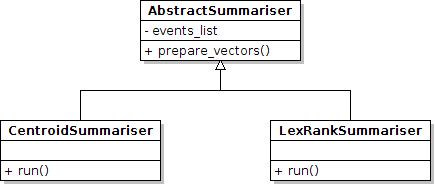
\includegraphics[height=2.0in, width=4in]{summarisers}
    \caption{The two derived summarisers share common functionality which is implemented in the AbstractSummariser class. }
    \label{SummariserArchitecture}
  \end{center}
\end{figure} 

\subsubsection{Centroid-based summariser}
The main idea behind this summariser is that tweets closer to the event's cluster centroid are more likely to be \emph{useful} and \emph{relevant} to the event than others which are distant. Also, the third criterion (quality) is met since the centroid's weights are calculated based on the average of the tweets' vectors and therefore typos and spelling mistakes are more likely to be ruled out. The implementation of this algorithm is straightforward and is shown in Listing \ref{CentroidSummariserSnippet}. First we retrieve the term-frequency vectors for all the documents in the cluster we want to rank. Then we calculate the centroid by averaging the individual vectors. Finally, the cosine similarity of each document and the centroid is calculated and we return a sorted list of similarities. The similarity acts as a ranking score since the closer a document is to a centroid the highest its ranking.  

\begin{lstlisting}[language=Python, label=CentroidSummariserSnippet, caption=Pseudocode for the centoid-based summariser.]
def run(event_cluster):
  '''
  Inputs:
  event_clusters: The cluster for which we want to rank 
                  the tweets.
  Outputs:
  ranked: A list of ranked tweets in descending order. 
  '''        
  vectors = event_cluster.get_document_vectors()
  
  #Calculates the centroid by averaging the individual
  #vectors of alll the documents in the cluster.
  centroid = calculate_centroid(vectors)
  
  similarities = []
  for vector in vectors:
    sim = cosine(vector, centroid)
    similarities.append(sim)
  
  return sorted(similarities)
  
\end{lstlisting}

\subsubsection{LexRank summariser}
As we have described in Chapter \ref{TheoreticalFramework} 
LexRank is an algorithm where we define a graph which consists of nodes representing the sentences in the text to be summarised and the 
edges are placed between two sentences that are similar to each other. We can then rank all the sentences 
based on the expected probability of a random walker visiting each sentence using equation \ref{LexRankEquation}. \\
The main difference between our implementation and the original LexRank algorithm is that we scale the probability of 
jumping to the next node based on the cosine similarity of two nodes. The reason for this is that we want to favor jumping to 
a node that discusses a more similar topic. We can implement this change by scaling the summation in the equation by the cosine similarity 
of the nodes $u$ and $v$. Since the similarity is in the range $[0, 1]$ an identical node it won't be discounted whereas a node with similarity equals 0 
it will be ignored. The equation the becomes:

\begin{eqnarray}\label{LexRankEquationModified}
L(u) = \frac{d}{N} + (1-d) * sim(u, v) \sum_{v \in adj[u]}^{\infty}\frac{L(v)}{deg(v)}
\end{eqnarray} 

\begin{lstlisting}[language=Python, label=CentroidSummariserSnippet, caption=Pseudocode for the centoid-based summariser.]
def run(event_cluster, threshold, tolerance):
  '''
  Inputs:
  event_clusters: The cluster for which we want to rank 
                  the tweets.
  Outputs:
  ranked: A list of ranked tweets in descending order. 
  '''        

  vectors = event_cluster.get_document_vectors()      
  n = len(vectors)
  adjacency_matrix,degree=calculate_similarities(vectors, 
                                              threshold)
  
  for i in xrange(n):
      for j in xrange(n):
        adjacency_matrix[i][j] = adjacency_matrix[i][j] 
                                            / degree[i]
                                            
  ranked = power_method(adjacency_matrix, tolerance)        
  
  return ranked
    
def power_method(self, m, epsilon):
  n = len( m )
  p = [1.0 / n] * n
  while True:
      new_p = [0] * n
      for i in xrange( n ):
          for j in xrange( n ):
              new_p[i] += m[j][i] * p[j]
      total = 0
      for x in xrange( n ):
          total += ( new_p[i] - p[i] ) ** 2
      p = new_p
      if total < epsilon:
          break
  return p  
\end{lstlisting}

\subsection{Named entity and keyword extraction}
The other two parts of the summarisation module is the named entity and keyword extraction. The keyword extraction task is straightforward since we merely
find the keywords in the event cluster that have the heighest TF-IDF weights. For the name entity extraction task we decided to use the built-in capabilities of NLTK. More specifically, NLTK contains functions which can implement part of speech tagging and then extract named entities based on these tags\footnote{The pseudocode for this task is not included since it has not been implemented by us.}. For example if the input to the system is a tweet with the following content: "Most protesters in Cairo have gathered in front of the Maspiro building, protest in Alex is also picking up ‪\#jan25" then the output will be "Cairo, GPE" meaning that Cairo is identified as a location. Named entity extraction is not always accurate and therefore we must be careful when we decide which entities to output. For example in the above tweet the system could erroneously identify the word "Alex" as a person's name. However, in reality the author of the tweet mentioned the city Alexandria in Egypt. Therefore, in order to minimise the possibility of a misinterpretation we decided to output only named entities that appear very frequently in a cluster. 

\section{Classifying users}
In our system user classification is an important feature since it can allows us to understand the events even better. In this section we describe the implementation of automatic classification of users. The motivation behind this is the fact that we would like to be able to filter tweets according to their authors. For example, we might want to extract events based only on tweets from journalists. Since we want to investigate the events that took place during the Arab Spring we know that the important types of users we need to consider are: Media organisations, Journalists, Activists, Celebrities and Common individuals. In order, to classify a user to one of these categories we must construct its profile. A user profile is an N-dimensional vector of attributes that are used to discriminate different user types. We have narrowed down these attributes to be:
\begin{itemize}
  \item Retweet ratio
  \item Tweets conatining links ratio
  \item How often does this user get retweeted?
  \item Ratio of replies
  \item Ratio of mentions
  \item Followers to followees ratio 
\end{itemize}
The first attribute is the number of retweets of a user divided by the overall number of their tweets. Retweets are mainly used by ordinary individuals to share a tweet they liked but they are rarely used by media organisations. Therefore, if the retweet ratio is very small we may suspect that this is a media organisation. The second attribute denotes the number of tweets containing links divided by the total number of tweets of a user. This is also an important feature because we can very easily identify a media organisation from the number of tweets that contain links. The reason is because Twitter accounts for media organisation are mainly used to share links of their articles. If a user gets retweeted too often this is usually an indication that they are popular or their tweets are considered interesting. Therefore, the number of times a user gets retweeted can be a measure of its popularity and therefore if we observe a user which gets retweeted frequently we may assume they are a celebrity, a journalist or even an activist. A user can reply to another user by using the "@" character followed by the username and the same holds for when a user wishes to mention another user in a tweet. The difference between a mention and a reply is that replies have the "@username" pattern in the beginning, whereas in mentions this pattern can appear anywhere. Replies are usually used by ordinary individuals to start and maintain conversations but are very rarely used by celebrities and media organisations. Finally, one of the most discriminating features is the followers to followees ratio. The reason for this is because celebrities and media organisations have very high followers to followees ratio while ordinary individuals have very low ratio. Activists and journalists are in the middle of the spectrum.\\\\
The task now becomes to collect a training dataset which contains labelled user profiles. This will be used to train our classifiers. The obvious way to collect the data is by manually looking up users on Twitter and constructing their profiles. However, this will be a tedious and time consuming process and thus we decided to collect our data automatically. We have achieved this by crawling a website called Twtrland \footnote{http://twtrland.com/} which provides Twitter user statistics.   

\subsection{Crawling user profiles}
A web crawler is a type of software agent that browses websites in a methodical and automated way in order to retrieve up-to-date information. This technique is used in our case to retrieve user profiles from Twtrland. Our web crawlers are constructed using an open source crawling library for Python called Scrapy \footnote{http://scrapy.org/}. A crawler is given the URL of a user profile on Twtrland and then it parses the HTML code of that page retrieving the information we need. A typical page on Twtrland is shown in Figure \ref{TwtrlandPage} and the red rectangles indicate the information we collect. 

\begin{figure}[htbp]
  \begin{center}
    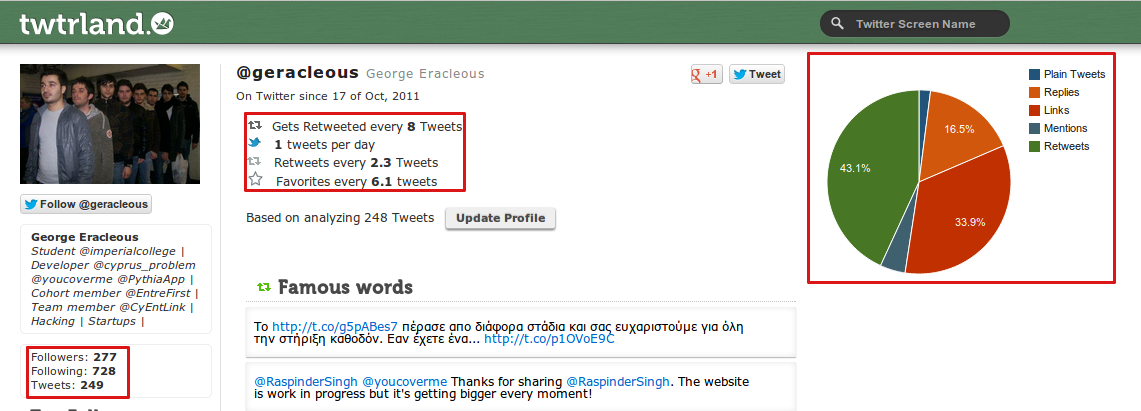
\includegraphics[height=1.9in, width=6in]{twtrland-page}
    \caption{A typical Twtrland user profile. The information in the circles is retrieved by our crawler and used in the construction of the user feature vector.}
    \label{TwtrlandPage}
  \end{center}
\end{figure} 

\subsection{Constructing the feature vectors}
Based on the information we have collected using our crawlers we can very easily construct a feature vector for each user. The vector has one column for each of the six attributes we 
defined above. Some examples of feature vectors are shown in Table \ref{FeatureVectors}. The columns represent the username, retweet ratio, link ratio, how often this user gets retweeted, replies ratio, mentions ratio and followers to followees ratio (FF) respectively. 

\begin{table}[htbp]
\footnotesize
\centering
\begin{tabular}{ l  l  l  l  l  l  l }
  \hline
  \textbf{User} & \textbf{Retweets} & \textbf{Links} & \textbf{Retweeted} & \textbf{Replies} & \textbf{Mentions} & \textbf{F/F} \\ \hline
  \emph{nytimes} & 0.0540 & 0.9091 & 0.6700 & 0.0043 & 0.0033 & 7089.2700 \\
  \emph{aplusk} & 0.0970 & 0.4042 & 0.5000 & 0.1971 & 0.0880 & 14151.1944 \\
  \emph{bencnn} & 0.2702 & 0.0974 & 0.4500 & 0.0988 & 0.0093 & 186.1068 \\
  \emph{alaa} & 0.2500 & 0.0407 & 0.8700 & 0.5120 & 0.0733 & 134.4679 \\
  \hline
\end{tabular}
\caption{The feature vectors of different types of users users}
\label{FeatureVectors}
\end{table}

\noindent The first user is the Twitter account of New York Times and it is representative of the feature vectors for media organisations. Low retweet rate and a large proportion of their tweets contain links as expected. Their Followers to Followees (FF) ratio is very high and one can easily infer by their low reply and mention ratii that they almost never engage in a conversation. The second example is Ashton Kutcher, a famous Hollywood actor. His FF ratio is very high, as expected, and another important observation is that his replies ratio is relatively high meaning that he usually chats with other users. The username bencnn belongs Ben Wedeman a famous American journalist working for CNN. An interesting observation is that his tweets are retweeted a lot. More specifically, he gets retweeted every 0.45 tweets which is the highest rate from all four examples. This is expected as he usually tweets content that people find interesting and worth sharing. Finally, the fourth example profile belongs to Alaa Abd El-Fattah, a well known Egyptian political activist. In his profile we can observe relatively low FF ratio but very high replies ratio which is expected as he usually engages in conversations with other users.

\subsection{Software architecture}
Figure \ref{Classifiers} depicts the software architecture of the user classification module. Once again we wanted to make it as easy as possible to swap implementations of classifiers and therefore
the AbstractClassifier class factors out the common functionality of classifiers leaving the concrete implementations to the derived classes. 

\begin{figure}[htbp]
  \begin{center}
    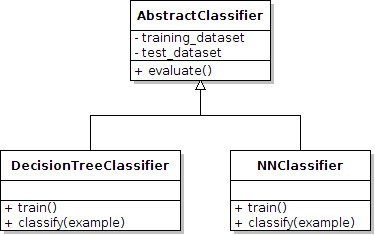
\includegraphics[height=2in, width=4in]{classifiers}
    \caption{The two derived classifiers share common functionality which is implemented in the AbstractClassifier class. }
    \label{Classifiers}
  \end{center}
\end{figure} 

\subsubsection{ID3 Classifier implementation}
One of the most popular decision tree learning algorithms is the ID3 and there are a lot of open source implementations. It learns a decision tree by constructing it top-down iteratively and 
at each iteration it tries to find the best attribute from the feature vector to be tested, i.e. the attribute that helps the most in discriminating the examples. It selects this attribute using
a statistical test to determine how well it classifies the training examples.\\\\
We consider decision trees to be an excellent choice in our case since they are less prone to noise in the data than other algorithms. Our dataset is likely to contain noisy user profiles since some of the user profiles are misleading due to the existence of automatic tweet bots and fake accounts. The effect of this noisy examples can be ruled out by the decision tree learning algorithm.  
We have decided to use Orange's ID3 implementation which can be easily extended to incorporate new functionality. In particular, in our implementation we have written wrapper functions for training and testing a classifier. We train the classifier with the labelled user examples we have collected using our crawlers and then using the learned tree we can classify unknown examples. A part of the learned tree based on our training dataset is shown in Figure \ref{Tree}. Leaf nodes in this tree are labelled with numbers in the range $[0, 4]$ where each number indicates a different type of user (0: Celebrity, 1: Media Organisation, 2: Journalist, 3: Activist, 4: Ordinary Individuals). ID3 selected the root node to be the FF ratio and this is expected since this attribute is usually enough to get an indication of the type of the user. If the FF ratio for an example is lower than 143.068 then we move to the left branch otherwise to the right one. We keep moving downwards the tree until we hit a leaf node which gives the final classification for this example. For instance if an example has FF ratio higher than 143.068, it gets retwetted in less than 0.070 tweets and the proportion of links in the tweets is lower than 0.043 then the we hit the leaf node labelled with the number $0$. This number indicates that the class of this example is "Celebrity".

\begin{figure}[htbp]
  \begin{center}
    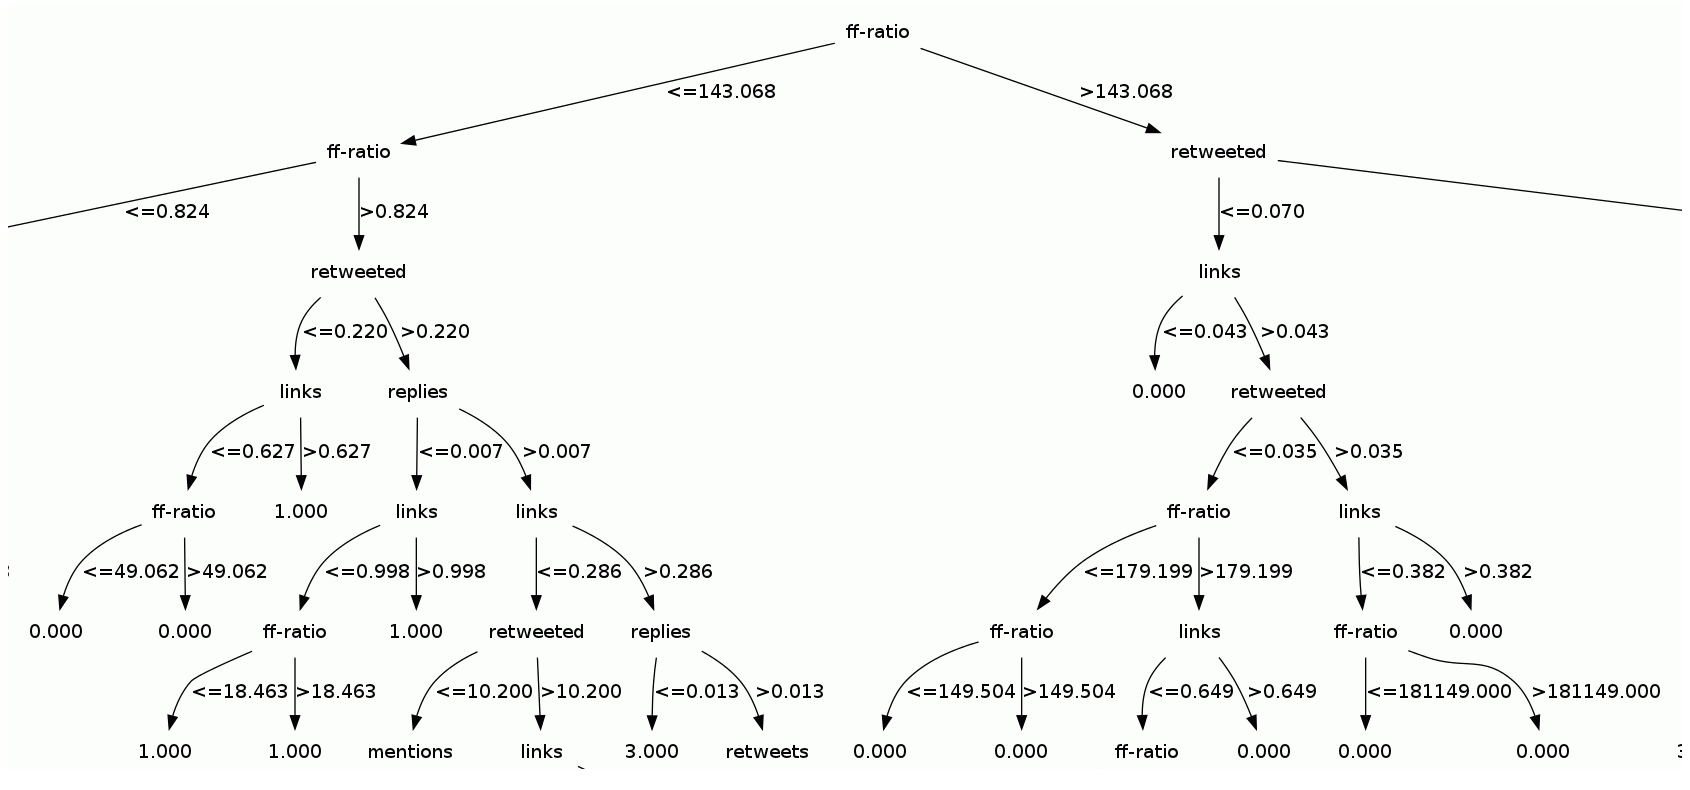
\includegraphics[height=3in, width=6in]{tree}
    \caption{Part of the decision tree learned by our classifier.}
    \label{Tree}
  \end{center}
\end{figure} 

\subsubsection{k-Nearest Neighbours Classifier implementation}
Another approach for classifying users is the k-Nearest neighbour which is again effective in handling noisy datasets given a relatively large training dataset. Once again we have used the k-Nearest neighbour algorithm implemented with Orange and in Chapter \ref{Evaluation} we compare its performance against the decision tree implementation. The algorithm receives the training data, in the same way as the ID3 algorithm does, and then we can present it with a new example to get its classification. As it is expected a lazy learning algorithm like k-Nearest neighbour takes longer to classify an example but much less time during training since effectively there is no training phase.   

\section{Summary}
This chapter presented the implementation of different subcomponents of a data mining toolset. The chapter's section proceeded step-by-step through all the stages of our methodology, from data retrieval and text preprocessing to clustering and summarisation. When the various components of this toolset are connected, they should construct an event detection and summarisation system. In the next chapter we evaluate the methods implemented in this chapter in order to find out which are performing best.
% ------------------------------------------------------------------------


%%% Local Variables: 
%%% mode: latex
%%% TeX-master: "../thesis"
%%% End: 

\chapter{Evaluation}\label{Evaluation}
\ifpdf
    \graphicspath{{Chapter4/Chapter4Figs/PNG/}{Chapter4/Chapter4Figs/PDF/}{Chapter4/Chapter4Figs/}}
\else
    \graphicspath{{Chapter4/Chapter4Figs/EPS/}{Chapter4/Chapter4Figs/}}
\fi
A number of different clustering and classification algorithms have been used in our implementation of the event extraction system. 
Some of them are more suitable for mining social media content and some others are not. In this capter we evaluate, both quantitatively and qualitatively, 
these algorithms based on real data collected from Twitter and we provide the results of several experiments we have conducted using this dataset. 
Our quantitative analysis consists of comparing the accuracy and the quality of the clusterers and the classifers as well as their runtime performance. 
Finally, based on our results we discuss and explain which algorithms pass the test and will be used in the development of 
proof-of-concept application in Chapter \ref{CaseStudy}.

\section{Document clustering evaluation}
Cluster analysis is the core component of our system and its evaluation is of great importance to us. We have implemented 
four different clustering algorithms and some of them have been used with success in traditional document clustering. However,
in our case we are asked to tackle an entirely different problem since we deal with social media content and the challenges that come with it. 
We have identified three major challenges that are inherent to tweets and our clustering evaluation evaluates quantitatively the individual merits and demerits 
of each algorithm with respect to these challenges. More specifically, the three major challenges are:

\begin{itemize}
   \item \textbf{Number of documents:} The first difference between traditional document clustering is that our system must operate on a vast amount 
   of tweets. In March 2011 Twitter reported that a billion tweets are sent per week [put reference Penner, 2011 here] and events that are getting a lot 
   of traction, such as the Arab Spring, will be associated with a huge number of tweets. Therefore, our first consideration is scalability and whether our algorithms can cope with the 
   number of tweets.    
   \item \textbf{Document length:} Tweets, unlike normal web documents, are very short and they are limited to 140 characters. Longer documents are, in general, more likely
  to contain more examples of the features of interest than shorter ones [put reference here Hermann Moisl ] hence clustering may be more accurate with longer documents. This fact may 
  affect the accuracy of our algorithms and we should investigate their relative performance. In our evaluation we use the average document length which is the sum of lengths of all documents 
  in the corpus divided by the number of documents. 
   \item \textbf{Vocabulary diversity :} Another major challenge due to the nature of the tweets is the diversity of the vocabulary used. Tweets are supposed to be informal documents
   and this greatly affects the quality of their content. For example, many tweets contain spelling mistakes, typos or abbreviations and sometimes users use words from multiple languages.
   Also, usually people tend to make small modifications to existing tweets and retweet them with the consequence that we collect several tweets that essentially have the same meaning but their
   vocabulary varies. This is a big concern for us since our clustering methods use the vector space representation which uses the word frequencies to find similarities. Hence the vocabulary 
   diversity will affect the term frequencies and consequently our results. We define vovabulary diversity as the number of distinct terms in a corpus divided by the number of documents in the corpus.
\end{itemize} 
What we try to achieve in the next sections is to evaluate our clustering algorithms by considering the three challenges describes above as variables. We vary these variables and 
record the performance of each algorithm in each case. In addition to these variables we also investigate the effect of different similarity measures on our results. 

   
\subsection{Data and evaluation methodology}\label{ClusteringEvaluationMethod}
Our aim is to measure the quality of a clustering algorithm and we have a few methods to choose from to achieve this. There are two categories of clustering evaluation methods and the choice depends
on whether a ground truth is available. The first category is the extrinsic methods which require the existence of a ground truth and the other category is the intrinsic methods. In general, extrinsic methods try to assign a score, $Q(C, C_g)$, to a clustering $C$, given the ground truth $C_g$, whereas intrinsic methods evaluate clustering by examining how well the clusters are separated and how compact they are [put reference data mining book here].\\\\ 
In our evaluation we decided to use an extrinsic method by constructing the ground truth using data from the Arab Spring. More specifically, we use the BCubed precision and recall metrics. The BCubed precion and recall metrics differ from the traditional precision and recall (described in section \ref{ClassifiersEvaluationMethod}) in the sense that clustering is an unsupervised learning technique and therefore we do not know the labels of the clusters beforehand. For this reason BCubed metrics evaluate the precion and recall for every example in a clustering on a given dataset according to the ground truth. The precision of an example is an indication of how many other examples in the same cluster belong to the same category as the example. The recall of an example reflects how many examples of the same category are assigned to the same cluster.\\\\ 
Formally, let $D = \{ 0_1,....,o_n \}$ be a set of examples, and $C$ be a clustering on $D$. Let $L(o_i)$ where $1 \leq i \leq n$ be the label of $o_i$ given by the ground truth, and $C(o_i)$ be the cluster identifier of $o_i$ in $C$. Then, for two examples, $o_i$ and $o_j$, where $i \neq j$, the \emph{correctness} of the relation between $o_i and o_j$ is defined by:

\begin{eqnarray}
Correctness(o_i, o_j) = \begin{cases}
                          1& \text{if $L(o_i) = L(o_j) \Leftrightarrow C(o_i) = C(o_j) $},\\
                          0& \text{otherwise}.
                        \end{cases}
\end{eqnarray} 

BCubed precision is defined as 

\begin{eqnarray}
Precision BCubed = \frac{ \sum_{i=1}^{n} \frac{\sum_{o_j:i \neq j, C(o_i)=C(o_j)}^{} Correctness(o_i, o_j)}{\Vert \{ o_j | i \neq j, C(o_i) = C(o_j)  \}  \Vert} }{n}
\end{eqnarray} 

BCubed Recall is defined as

\begin{eqnarray}
Recall BCubed = \frac{ \sum_{i=1}^{n} \frac{\sum_{o_j:i \neq j, L(o_i)=L(o_j)}^{} Correctness(o_i, o_j)}{\Vert \{ o_j | i \neq j, L(o_i) = L(o_j)  \}  \Vert} }{n}
\end{eqnarray} 
While recall and precision can be used to determine the quality of a classifier, the usual approach is to combines the recall and precision rates in a single equation and this is 
achieved using the $F$ metric which is defined as:
\begin{eqnarray}
F = \frac{2 \times precision \times recall}{precision + recall}
\end{eqnarray} 
    
\subsection{Results}
For the construction of the ground truth we have manually labelled/categorised 285 tweets according to the events they described. In this dataset we have identified 35 different events. These tweets are collected using our data retrieval module and they are related to the Egypt's uprising. More specifically, these tweets describe the events that took place during a 2-hour period (12pm - 14pm) on 25th of January 2011.    

\subsubsection{Clustering quality vs Number of documents in the dataset}\label{EvalDiffNoDocs}
In this section we investigate the performance of the four different algorithms when the number of documents in our dataset varies while the other variables, the document length and the vocabulary diversity are kept constant. More specifically, we start with a small dataset of 50 documents and we iteratively add more documents (5 each time) until we reach a dataset size of 285. The average document length is $116.44$ characters/document and the vocabulary diversity is $1.07$ words/document. Also, the optimal parameters for the four classifiers are:

\begin{itemize}
  \item \textbf{k-Means:} The number of clusters, $k$, is set to 35 since we expect 35 events to be found. 
  \item \textbf{DBSCAN:} The two parameters needed for DBSCAN are set to $ε=0.5$ and $min\_pts=5$. 
  \item \textbf{NMF:} The number of bases is 35 since we expect 35 events (bases).
  \item \textbf{Online:} The window size is set to one third of the dataset size at any iteration. 
\end{itemize}\vspace{15pt}
We run three different experiments, each one with a different similarity metric. The results we obtained are illustrated in Figure \ref{DifferentSizeResults}

\begin{figure}[htbp]
  \begin{center}
    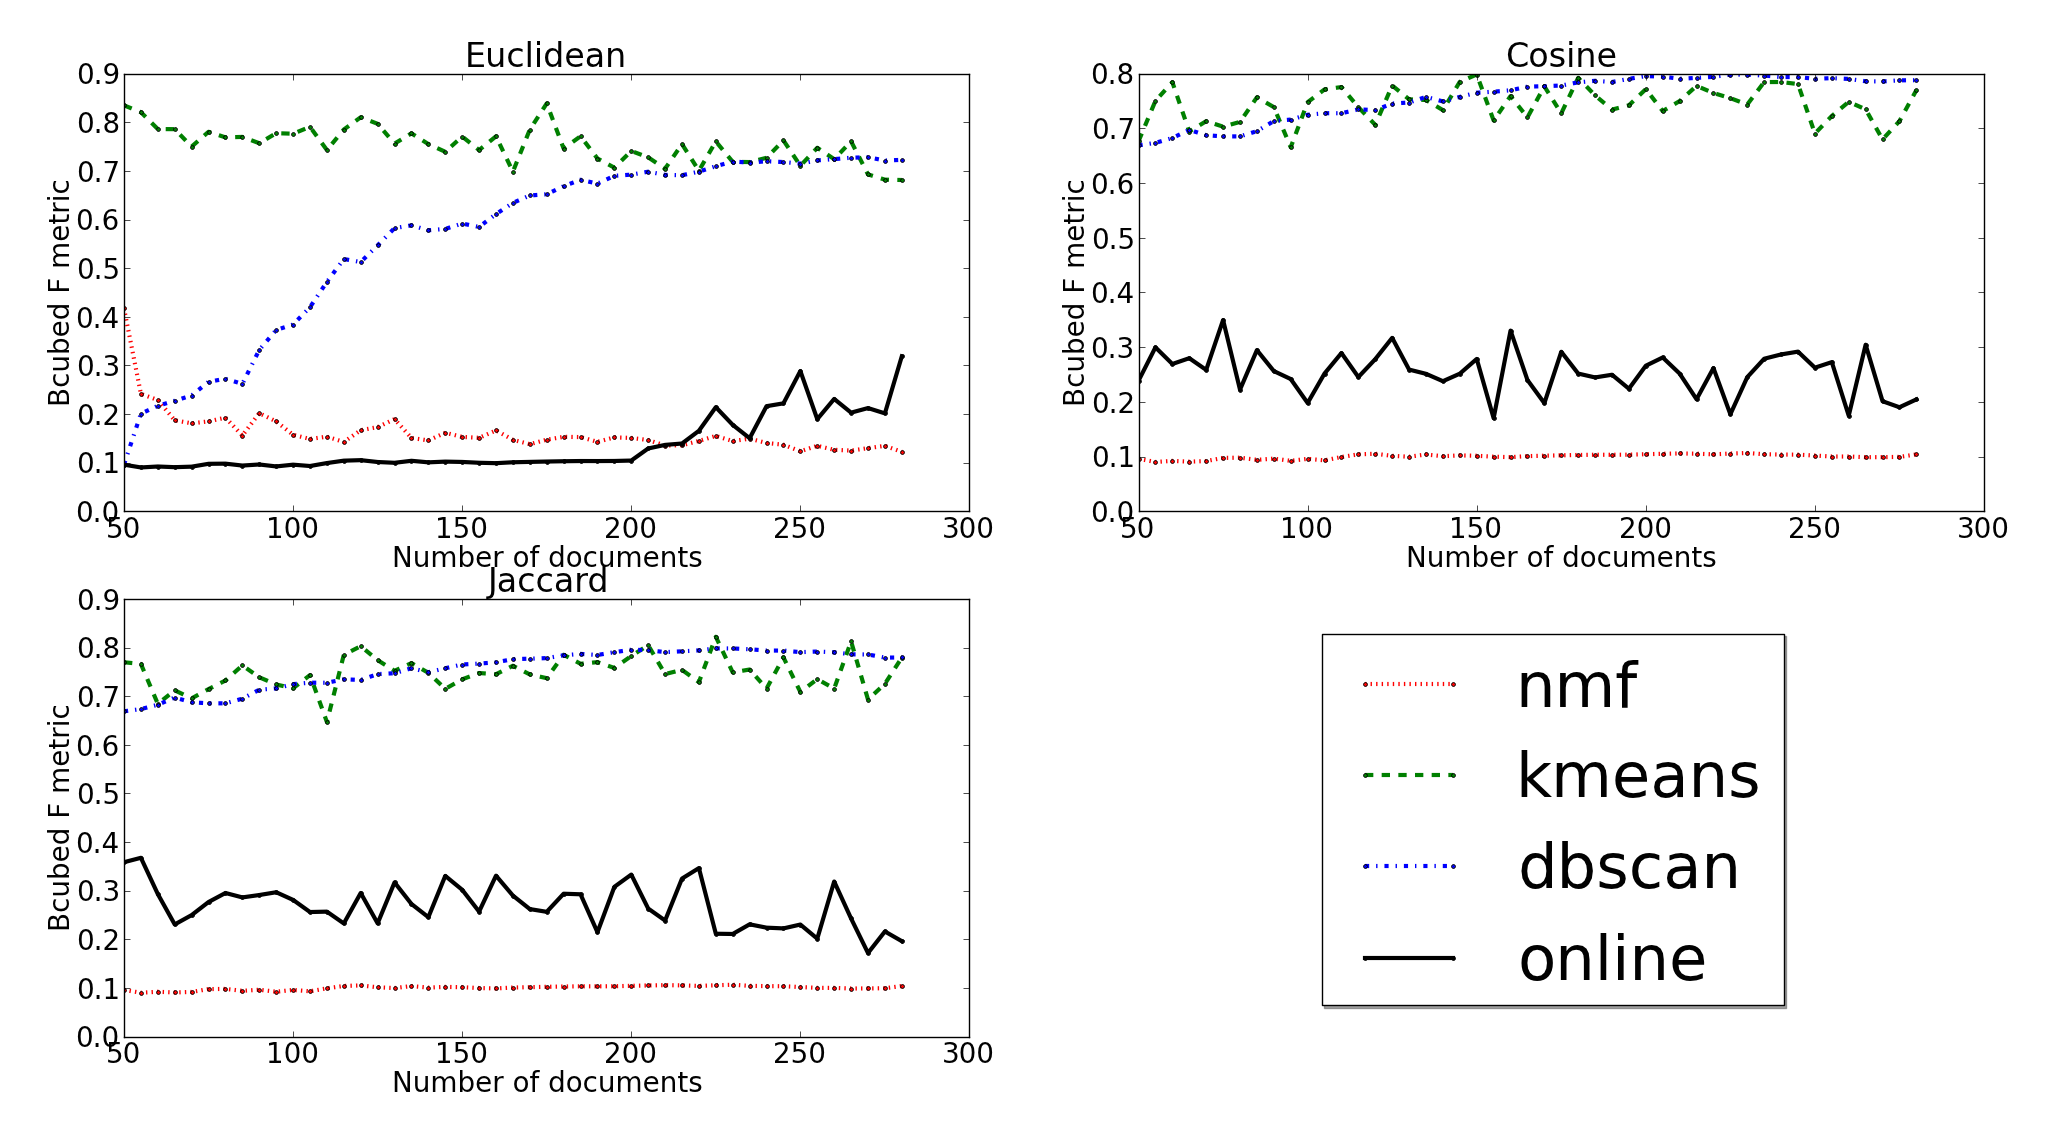
\includegraphics[height=5in, width=6in]{number_of_documents}
    \caption{Each plots depicts the results obtained using a different similarity metric. In each plot we illustrate the BCubed F metric (y-axis) against the number of documents (x-axis) of each clusterer.}
    \label{DifferentSizeResults}
  \end{center}
\end{figure}
The first important observation is that in all the plots DBSCAN and k-Means clusterers outperform the others in terms of the BCubed F metric. In all three cases k-Means performance is constantly around 0.8 although in the case of Euclidean distance the performance has a slightly negative trend as the number of document increases. On the other hand, DBSCAN initially has very low performance but as the number of documents increases the performance becomes better. A possible explanation is offered in [put reference 4 in pramata] which states that a disadvantage of DBSCAN algorithm is that it cannot cluster datasets well with large differences in density. Initially, the dataset is not very dense since the number of documents is small. However, as the number of document increases the performance increases too. The same scenario is depicted in the cases of cosine and Jaccard similarities. The only difference is that this time the initial performance of DBSCAN is not as low as for the Euclidean case.\\\\
The performances of the other two clusterers are much lower with the NMF clusterer having the lowest performance. The low performance of the online clusterer is expected since we have sacrificed accuracy for execution time performance by considering a limited window size. We have mentioned before that the term-frequency matrix for an online clusterer is constructed using only the last $N$ documents where $N$ is the window size. Therefore, any documents before this are lost and the TF-IDF weightings in the matrix are not accurate. A possible solution would be to use an approach similar to a moving average where the new TF-IDF weightings are calculated based on all the previous information plus the new information coming into the system.   

\subsubsection{Clustering quality vs Average document length}
In this experiment our aim is to evaluate our clusterers with different average document lengths in the corpus. We try to emulate the cases when a dataset conatins short documents and when it contains very long documents. Also, we want to find what happens in between these two cases. The motivation behind this experiment is that Twitter corpora are very short and we hypothesize that short documents yield worse results in terms of clustering quality.\\\\
We start with our original dataset which is described above and we incrementally add more words in the documents to deliberately increase their lenght. However, we have to keep the other two variables of our experiments constant. The number of documents is constant at 285 documents and in order to keep the vocabulary diversity constant, at $1.07$ words/document, the words that are appended to the documents are words that already belong to the dataset. Therefore, we achieve an increase in the document length without changing the vocabulary diversity. The initial value for the average document length is $116.44$. The clusterers use the same parameters as in Section \ref{EvalDiffNoDocs}. Again we have run three experiments with each one using a different similarity measure.\\\\  
\begin{figure}[htbp]
  \begin{center}
    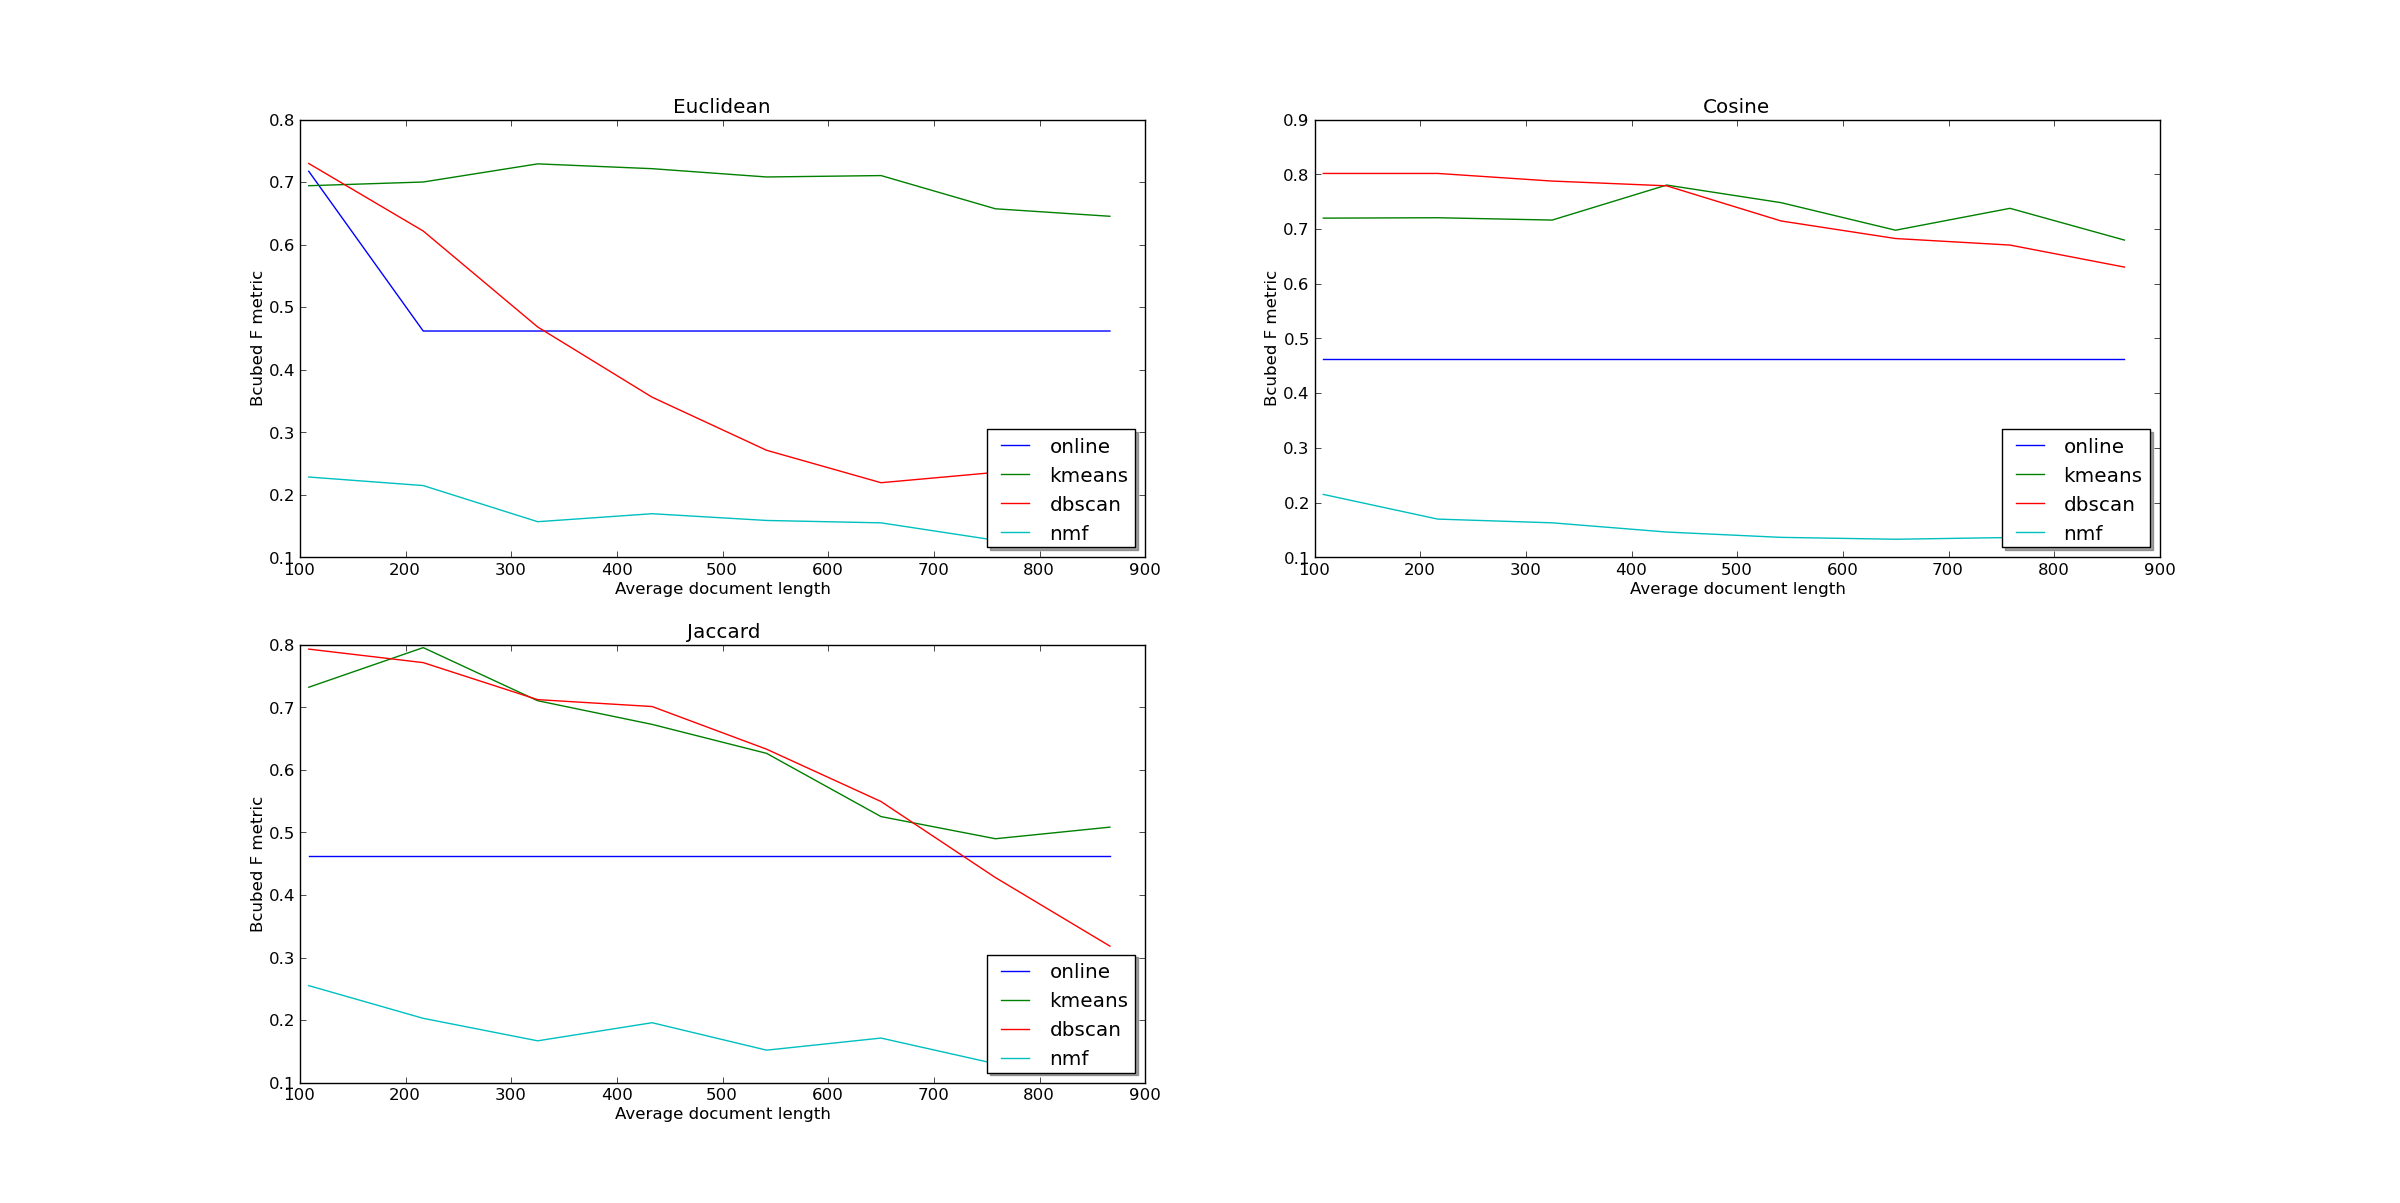
\includegraphics[height=5in, width=6in]{average_document_length}
    \caption{Each plots depicts the results of the experiment with a different similarity measure.}
    \label{DifferentLengthResults}
  \end{center}
\end{figure}
The results show that the performance of the classifiers is not greatly affected by the average document document length. Although, our hypothesis was that longer documents will aid the clustering process this turns out to be wrong. In our case the performance remains almost the same and in some cases exactly the same. However, we can clearly see that DBSCAN has the highest BCubed F score except for large document lengths in the Euclidean plot. The next best performing is k-Means and then online and NMF clusterers are once again inferior in performance.    


\subsubsection{Clustering quality vs Vocabulary diversity}
The final experiment is concerned with vocabularity diversity which is the number of distinct words in a dataset over the number of documents in it. Twitter corpora have a large vocabulary diversity due to the fact that they contain typos, spelling mistakes and abbreviations. In order to fabricate datasets with variable number of vocabulary diversity we employ a dictionaty of the English language. More specifically, we begin with our original dataset and in the next iteration we replace some of the words in the documents by random English words starting from a letter in the alphabet. In the next iteration we replace the words with others from the set of words starting from 2 distinct letters of the alphabet. This process continues, increasing the vocabulary diversity each time until we use all the 26 letters of the English alphabet. Also, notice that we replace some of the words in the original documents in order to keep the average document constant at $116.44$. The number of documents also remains constant at 285 documents. The parameters for the clusterers are the same as in Section \ref{EvalDiffNoDocs}. The results for the three different similarity measures are shown in Figure \ref{DifferentVocabularyResults}.\\\\ 
\begin{figure}[htbp]
  \begin{center}
    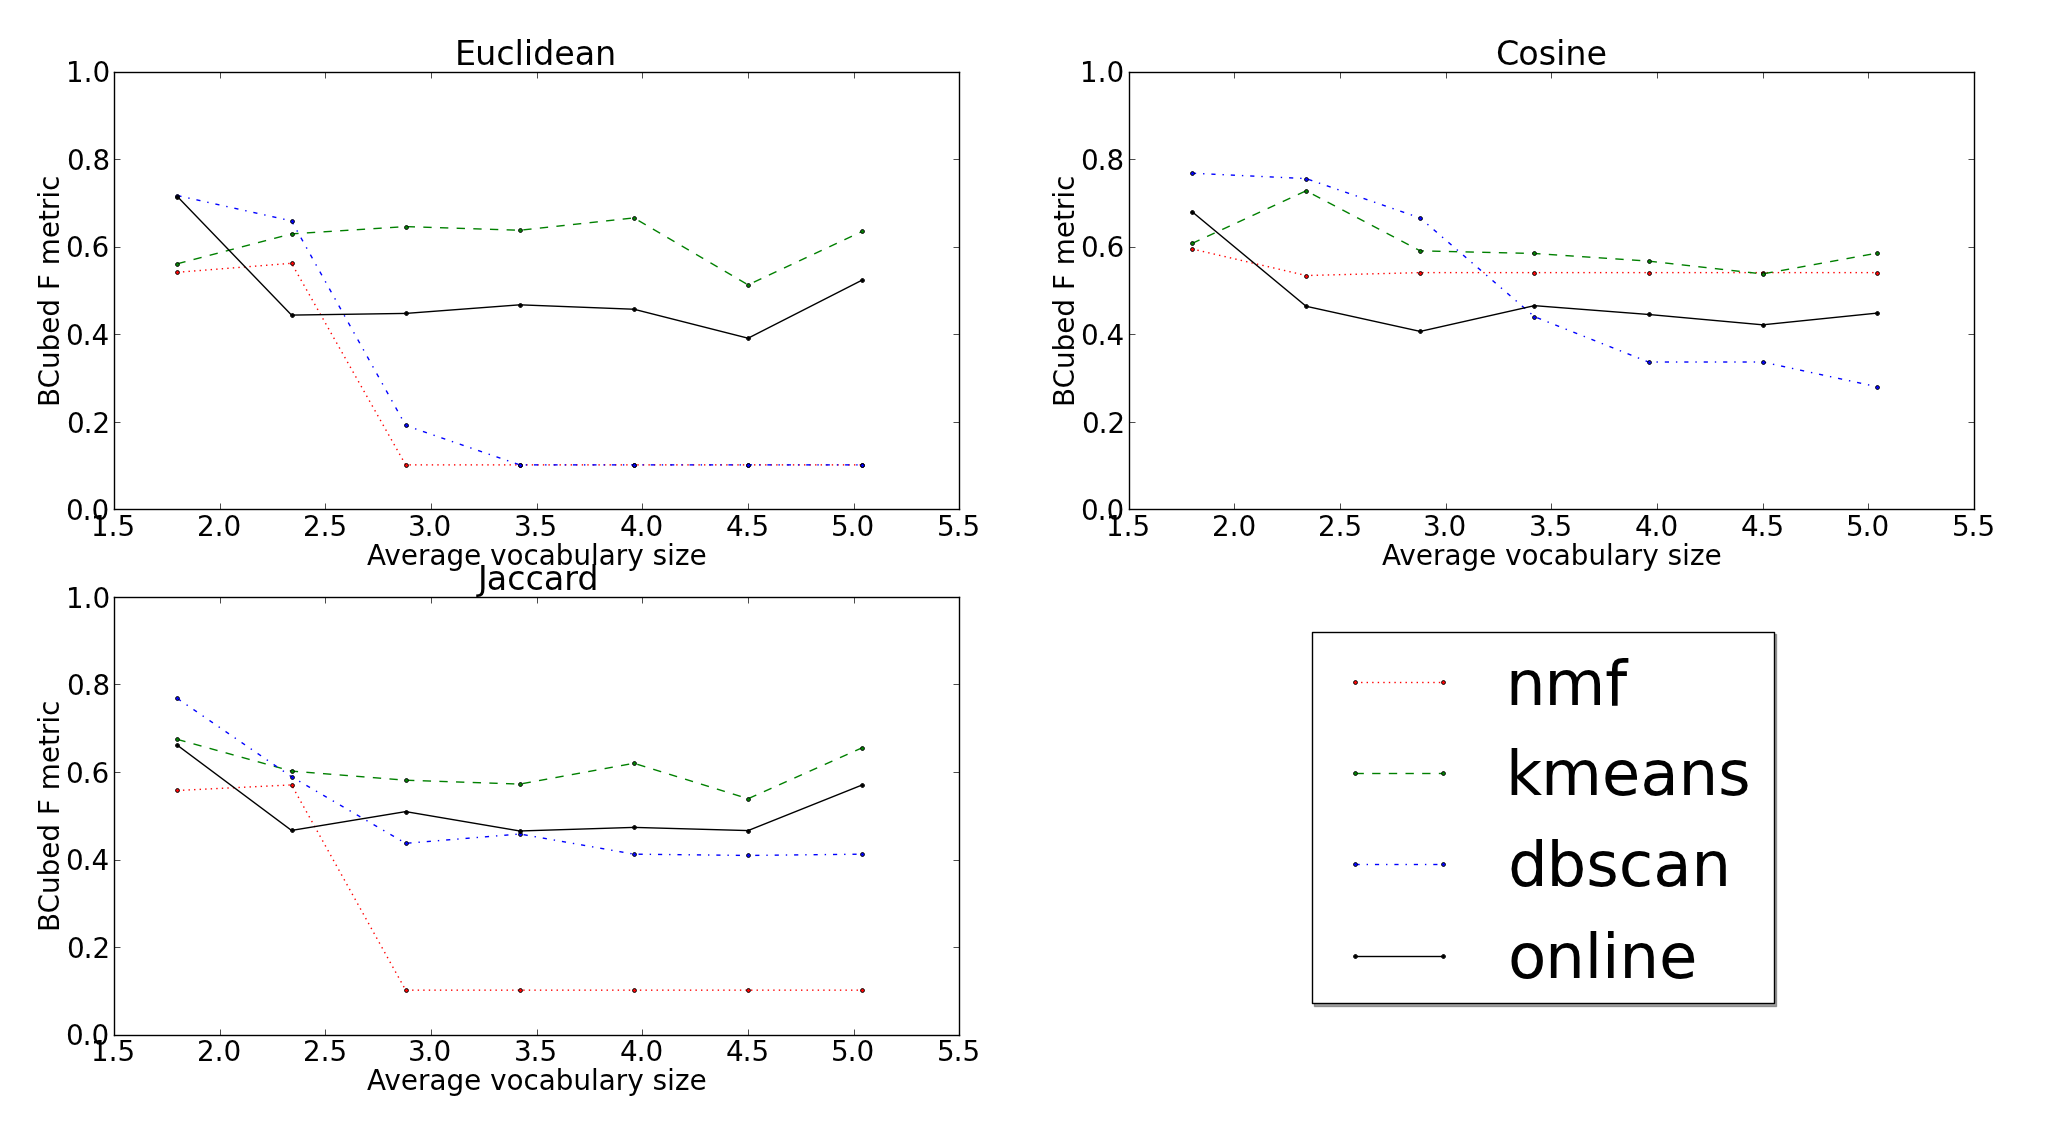
\includegraphics[height=5in, width=6in]{vocabulary}
    \caption{Each plots depicts the results obtained using a different similarity metric. In each plot we illustrate the BCubed F metric (y-axis) against the vocabulary diversity (x-axis) of each clusterer.}
    \label{DifferentVocabularyResults}
  \end{center}
\end{figure}
A first look at the results reveals that once again DBSCAN and k-Means algorithms have higher BCubed F scores than the other two. The overall trend in the plots indicates that in general as the vocabulary diversity increases the BCubed F score decreases for all clusterers, except from NMF's score which remains almost constant. An increase in vocabulary diversity means that it is harder to compute similarities between the documents since their common features are fewer. However, for the case of the cosine similarity we can see that the performance of DBSCAN and k-Means is immune to higher vocabulary diversities. The reason might be that due to the very diverse vocabulary the term-frequency vectors are very long and sparse since they contain many 0 values. Unlike the Euclidean distance, cosine similarity ignores these 0 values and focuses only on the common words between two documents and thus leads to better results.\\\\
The lower performance in this experiment stems from the fact that the feature vectors are getting larger due to the vocabulary diversity. Therefore, the dimensionality of the space becomes bigger and bigger and the effects of the "curse of dimensionality" reduce the performance of our clusterers. There are some remedies for this problem and one of them is to reduce the dimensionality by feature selection methods. One of these methods is Principal Component Analysis (PCA) that searches for $k n-dimensional$ orthogonal vectors that can best be used to represent the data, where $n$ is the dimensions of the feature vector and $k < n$[put reference data mining book]. We have used Orange's package for PCA and we have applied this dimensionality reduction methods on our two best clusterers. The results are shown in Figure \ref{DifferentVocabularyPCAResults}.\\\\ 
\begin{figure}[htbp]
  \begin{center}
    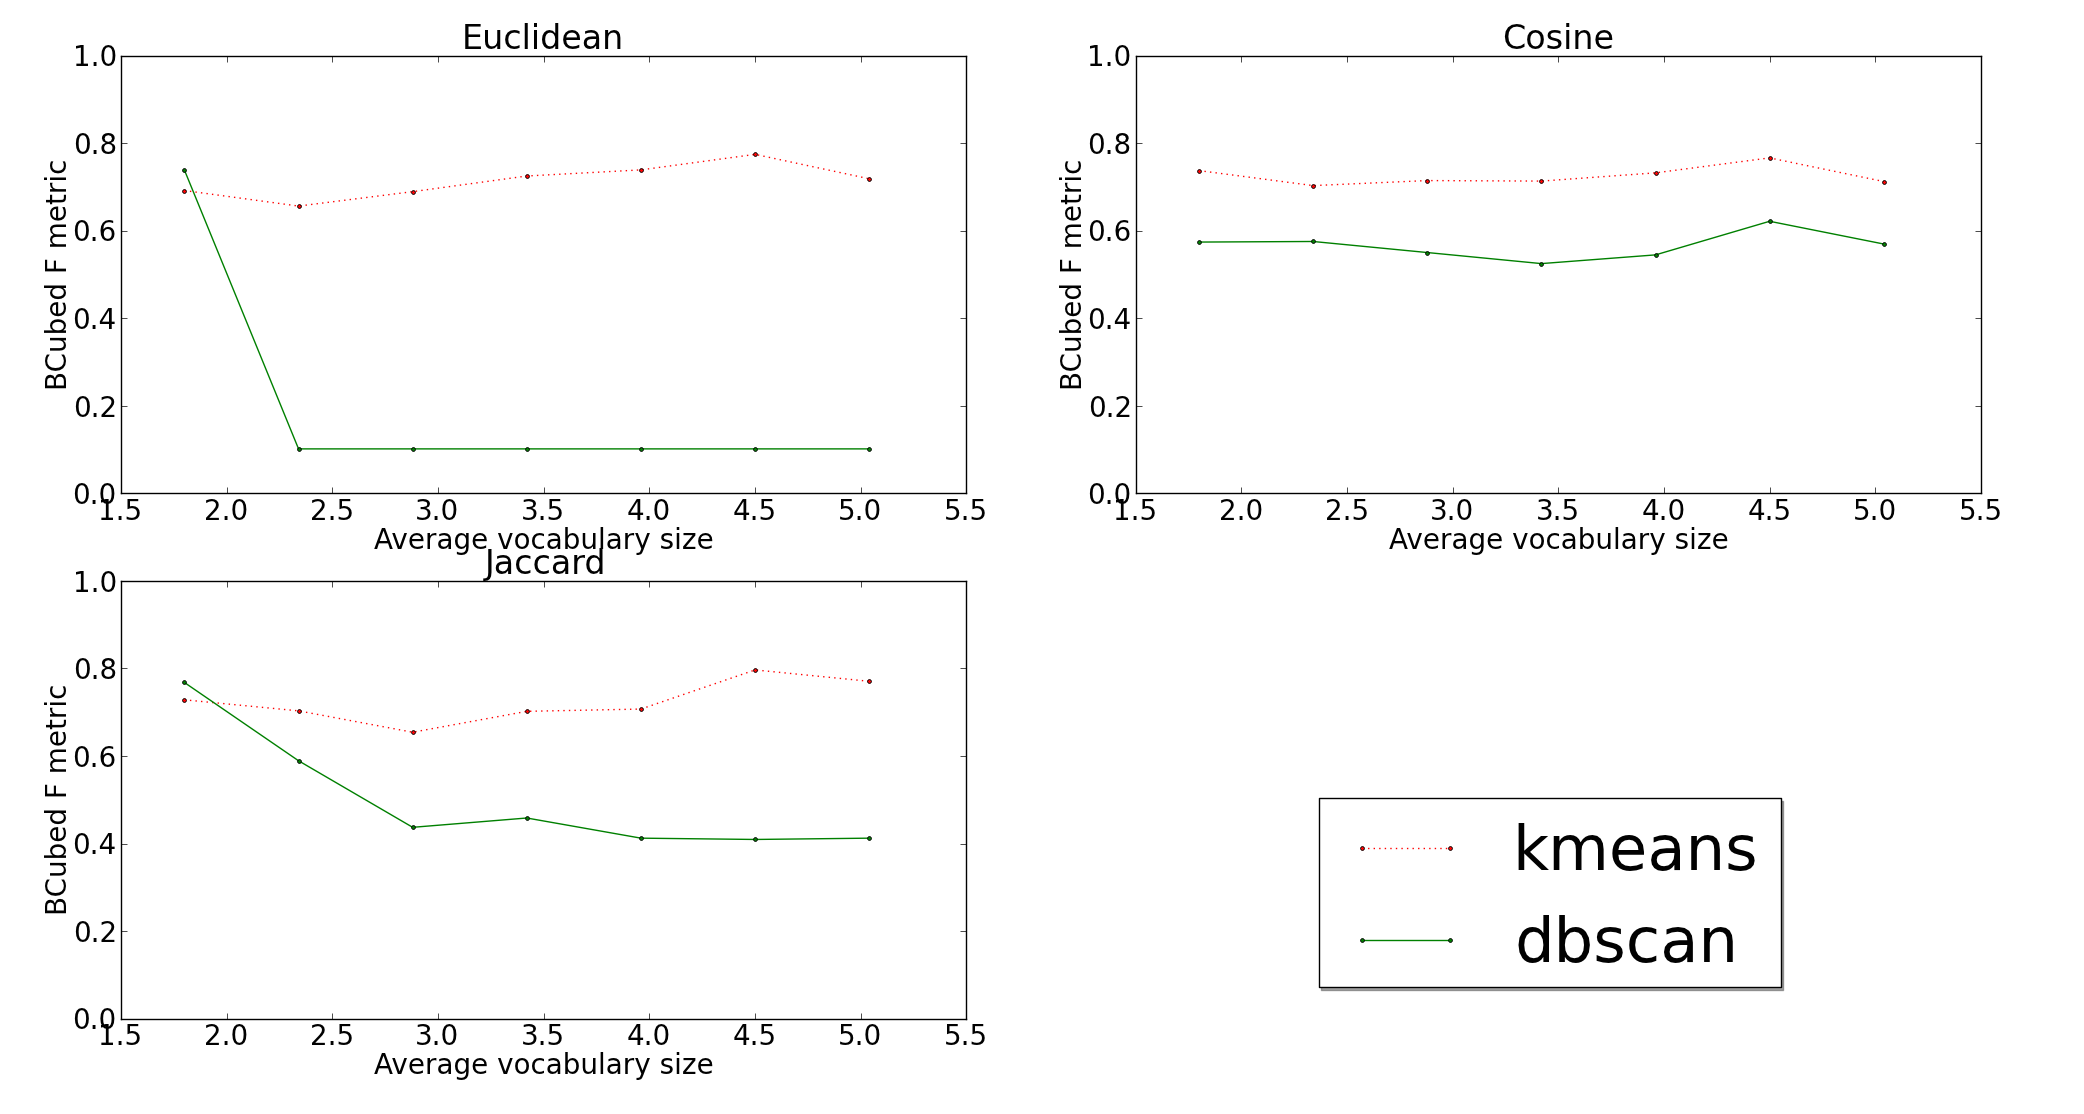
\includegraphics[height=5in, width=6in]{vocabulary_pca}
    \caption{The results for the BCubed F score against the vocabularty diversity after PCA have been used to reduce the dimensionality.}
    \label{DifferentVocabularyPCAResults}
  \end{center}
\end{figure}
The results are positive since the BCubed F score of k-Means has not only risen but it demonstrates a positive trend in all cases. DBSCAN's score remains the same for the Euclidean and Jaccard cases but it is improved for the case of cosine similarity. The initial score might be lower than the previous case but it never falls below $0.5$. Therefore, PCA can help in this case especially for k-Means.

\subsubsection{Execution time performance}
\begin{center}
\begin{tabular}{ | l | l| l | l | }
  \hline
  \textbf{Clustering method} & \textbf{Euclidean} & \textbf{Cosine} & \textbf{Jaccard} \\ \hline
  k-Means \begin{tabular}{ | r  }  Number of documents  \\ Document Length \\ Vocabulary Diversity \end{tabular} & 1 & 2 & 3 \\
  DBSCAN  \begin{tabular}{ | r  }  Number of documents  \\ Document Length \\ Vocabulary Diversity \end{tabular} & 1 & 2 & 3 \\
  NMF     \begin{tabular}{ | r  }  Number of documents  \\ Document Length \\ Vocabulary Diversity \end{tabular} & 1 & 2 & 3 \\
  Online  \begin{tabular}{ | r  }  Number of documents  \\ Document Length \\ Vocabulary Diversity \end{tabular} & 1 & 2 & 3 \\
  \hline
\end{tabular}
\end{center}

\section{Twitter user classification evaluation}

\subsection{Evaluation methodology}\label{ClassifiersEvaluationMethod}
In this section our aim is to identify which one of our classification algorithms performs better in terms of classification accuracy. Our classifier evaluation process involves the precision and recall metrics as well as the $F_1$ score. The precision and recall metrics definitions in this section are different from the ones described in section \ref{ClusteringEvaluationMethod} since classification is a supervised learning method and we can calculate these metrics using the labels of that training dataset. More specifically, precision can be thought as a measure of what percentage of examples that are classified by a classifier in a certain class are actually members of that class. On the other hand recall is a measure of what percentage of the overall population of examples belonging to a certain class have been classified by the classifier in that particular class. Formally, precision and recall are defined as:

\begin{eqnarray}
precision = \frac{TP}{TP + FP}
\end{eqnarray}  

\begin{eqnarray}
recall = \frac{TP}{TP + FN}
\end{eqnarray}  

where 

\begin{itemize}
  \item True Positives ($TP$): These are the positive tuples that were correctly labelled by our algorithm. 
  \item True Negatives ($TN$): These are the negative tuples that were correctly labelled by our algorithm.
  \item False Positives ($FP$): These are the negative tuples that were incorrectly labelled as positive by our algorithm.
  \item False Negatives ($FN$): These are the positive tuples that were incorrectly labelled as negatives by our algorithm.
\end{itemize}\vspace{15pt}

\subsection{Results}

In order to carry on our evaluation we have crawled 200 user profiles from Twtrland and labelled them manually according to the five user categories (celebrities, media organisations, journalists, activists and common people). During the process of labelling we made sure that the training dataset was as unambiguous as possible. However, in some cases the choice was not clear especially for the journalists and activists, since these two categories both overlap. A number of journalists usually are known to be activists as well. Finally, in order to produce as accurate results as possible we have used 10-fold cross validation. Cross-validation is the statistical practice of partitioning a sample of data into subsets such that the classifiers accuracy is tested on a single subset, while the other subsets are used for training. Since we have used 10-fold cross validation we split our dataset in subsets of 20 examples and 180 are used for training while the rest are used to test the classifier.\\\\
Figure \ref{DifferentClassifiersResults} demonstrates the average results of running 10-fold cross validation 100 times. Information gain is used as the statistical measure for selecting tree nodes in ID3 and post-pruning of the trees takes place after training in order to minimise the effects of overfitting. Also, for the k-nearest neighbor algorithm we have used Euclidean distance to measure similarity between examples and $k=10$ (10 nearest neighbors have given the best results in our dataset). 

\begin{figure}[htbp]
  \begin{center}
    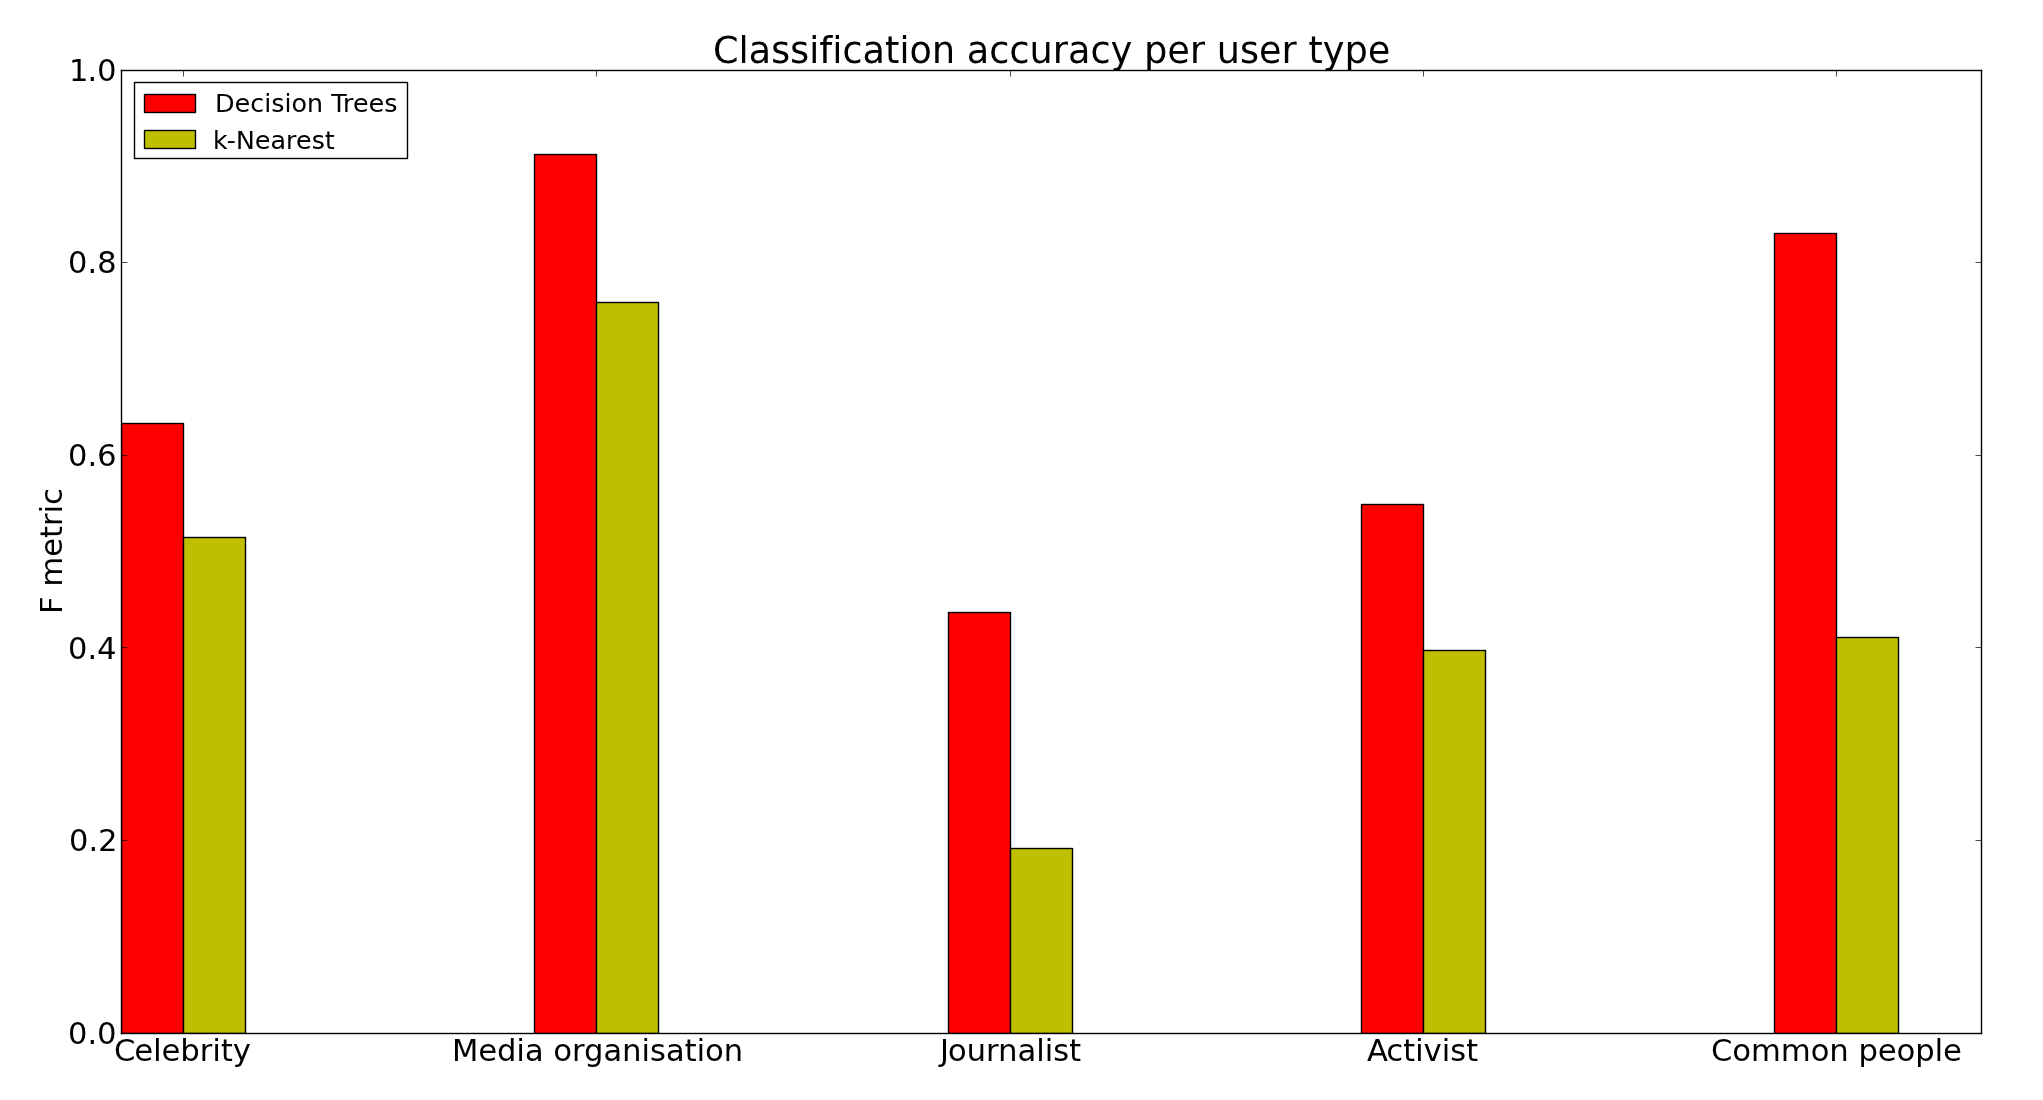
\includegraphics[height=5in, width=6in]{classifiers_bad}
    \caption{The F metrics obtain after 10-fold cross validation on our dataset for the two classifiers.}
    \label{DifferentClassifiersResults}
  \end{center}
\end{figure}
The results reveal that for all the classes the performance of the decision tree learning algorithm is better compared to the k-nearest neighbor learning. We attribute the differences in the results in two factors. First of all k-nearest neighbors algorithm is highly effective in cases when it is given a sufficient amount of training data. In our case due to the time-consuming process of collecting and manually labelling user profiles we have provided a small amount of training examples. The second problem is that since the user feature vectors are constructed based on a user's activity on Twitter we expect to have some outliers indicating irregular activity from some users (i.e. a celebrity having a small followers-to-followees ratio because they follow back almost everyone). These outliers can reduce the performance of a k-nearest neighbor classifier but we can use a weighted version of the algorithm where the effect distant examples is negligible. Additionally, unlike decision trees, the classification decision is based on all the attributes of the feature vector (Euclidean distance uses the whole vector length to calculate the distance). However, usually only a subset of these attributes are relevant for classification and therefore a similarity measure based on many irrelevant features might be misleading.\\\\ 
Based on the hypothesis that distance-weighted nearest neighbor algorithm can improve the performance we have changed our implementation to take into account the weights of each neighbor and the results are shown in Figure \ref{DifferentClassifiersResultsImproved}. It is obvious that the effect of outliers was significant in the case of common people since we can see an improvement over the old implementation.\\\\
A very important observation is the fact that for both classifiers the two classes with the lowest F score are the journalists and activists. This was expected because these two classes overlap significantly. Even for a human is difficult to distinguish between a journalist and an activist since sometimes some journalists are also activists. Finally, media organisations have the highest F score and again this was expected because they have some discriminating characteristics which can easily separate them from the other classes. Since these accounts act on behalf of huge organisations they do not act as human but more like a bot. For example, they almost never engange in conversation nor they retweet.  

\begin{figure}[htbp]
  \begin{center}
    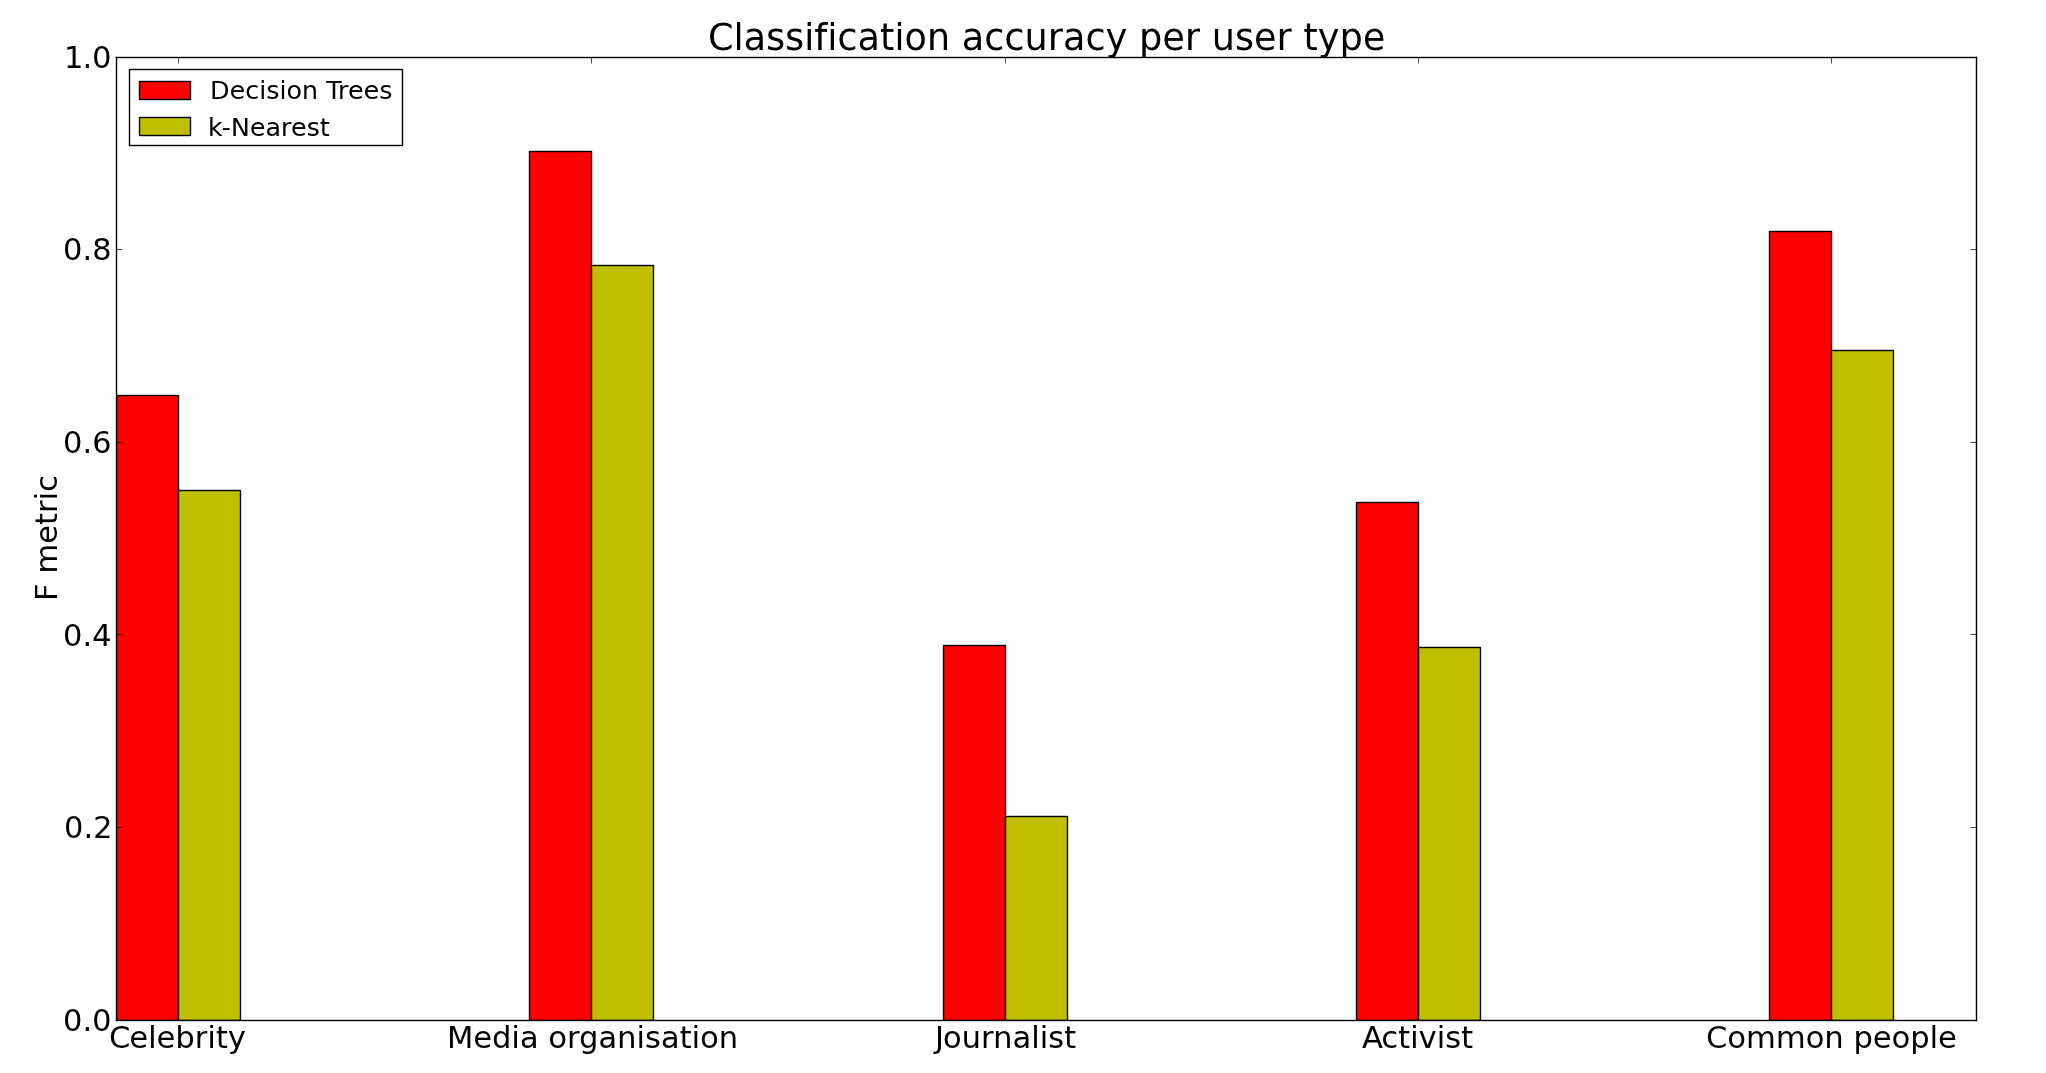
\includegraphics[height=5in, width=6in]{classifiers}
    \caption{The F metrics obtain after 10-fold cross validation on our dataset for the two classifiers.}
    \label{DifferentClassifiersResultsImproved}
  \end{center}
\end{figure}

\section{Optimisations}
Briefly explain how we improbed the execution time

\section{Summary}

% ------------------------------------------------------------------------


%%% Local Variables: 
%%% mode: latex
%%% TeX-master: "../thesis"
%%% End: 

\chapter{Pythia - An event exploration web application}\label{Pythia}
\ifpdf
    \graphicspath{{Chapter5/Chapter5Figs/PNG/}{Chapter5/Chapter5Figs/PDF/}{Chapter5/Chapter5Figs/}}
\else
    \graphicspath{{Chapter5/Chapter5Figs/EPS/}{Chapter5/Chapter5Figs/}}
\fi

\section{Pythia - An event exploration web application}\label{WebApp}
Our work in the previous chapters has led to the development of a proof-of-concept web application which can be used to extract and explore
events from Twitter. Pythia can be thought as the last module in the system overview in Figure \ref{SystemOverview}. It provides a graphical user interface that helps humans visualise the results of event detection and summarisation. The main motivation behind the development of this application is to demonstrate the capabilities of our work by looking at historical Twitter data from the Egypt uprising.\\\\
In the next section we describe how the application is built and how it can be used and the rest of the chapter shows the output of Pythia from Egypt's dataset.    

\subsection{Pythia's architecture and design}
The two core components of Pythia is the back-end side which is the data mining system that detects and summarises the events and the front-end side which is the graphical user interface responsible for accepting the user input and visualising the results. Pythia's back-end is built using a scalable, non-blocking web server called Tornado \footnote{http://www.tornadoweb.org/}. This web server is responsible for handling all the request from the front-end and returning the results back. Figure \ref{PythiaOverview} illustrates a very simple diagram of the application. First the front-end receives the user input which is a list of keywords describing the topic the user wants to explore. The list of keywords is passed to the back-end via a HTTP request and a handler is responsible to serve the request. It sends the list of keywords to a data processing module which is nothing more than our event detection system. Our system retrieves the relevant tweets from the database and performs event detection and summarisation. The results are passed by the handler back to the Pythia client and are presented to the user. 

\begin{figure}[htbp]
  \begin{center}
    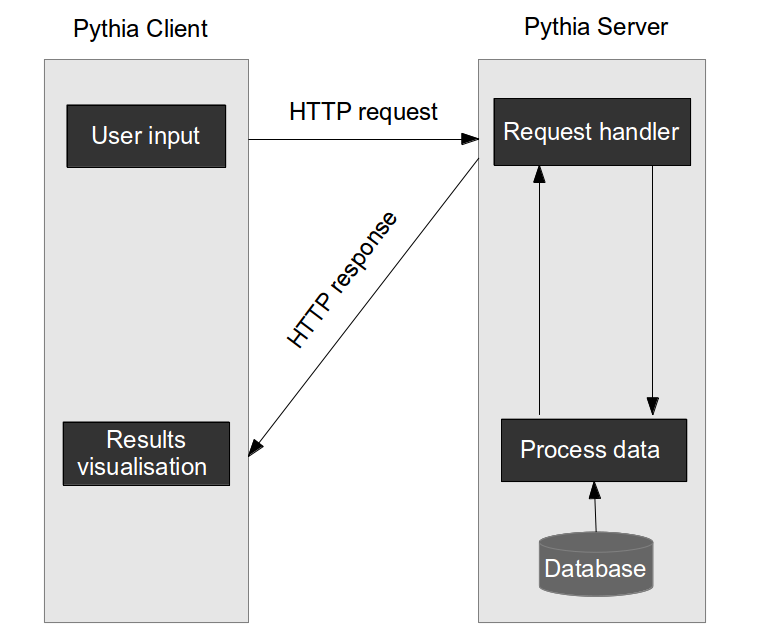
\includegraphics[height=5in, width=6in]{pythia-overview}
    \caption{An overview of Pythia's client-server architecture.}
    \label{PythiaOverview}
  \end{center}
\end{figure} 

\subsection{The Graphical User Interface (GUI) of Pythia}
The motivation behind Pythia is that we wanted to make it as simple as possible for a human to explore and understand events from a Twitter dataset. Therefore, throughout  
the development of Pythia our main consideration was to keep the GUI as lean and simple as possible. The simplicity should not come at the expense of information consumption therefore
another consideration was to give to the user as much information as possible.\\\\
When a user launches Pythia the first page that appears is the one shown in Figure \ref{Pythia1}. A simple text box is used receive the list of keywords provided by the user. The keywords are used to retrieve tweets that contain these words.\\\\
\begin{figure}[htbp]
  \begin{center}
    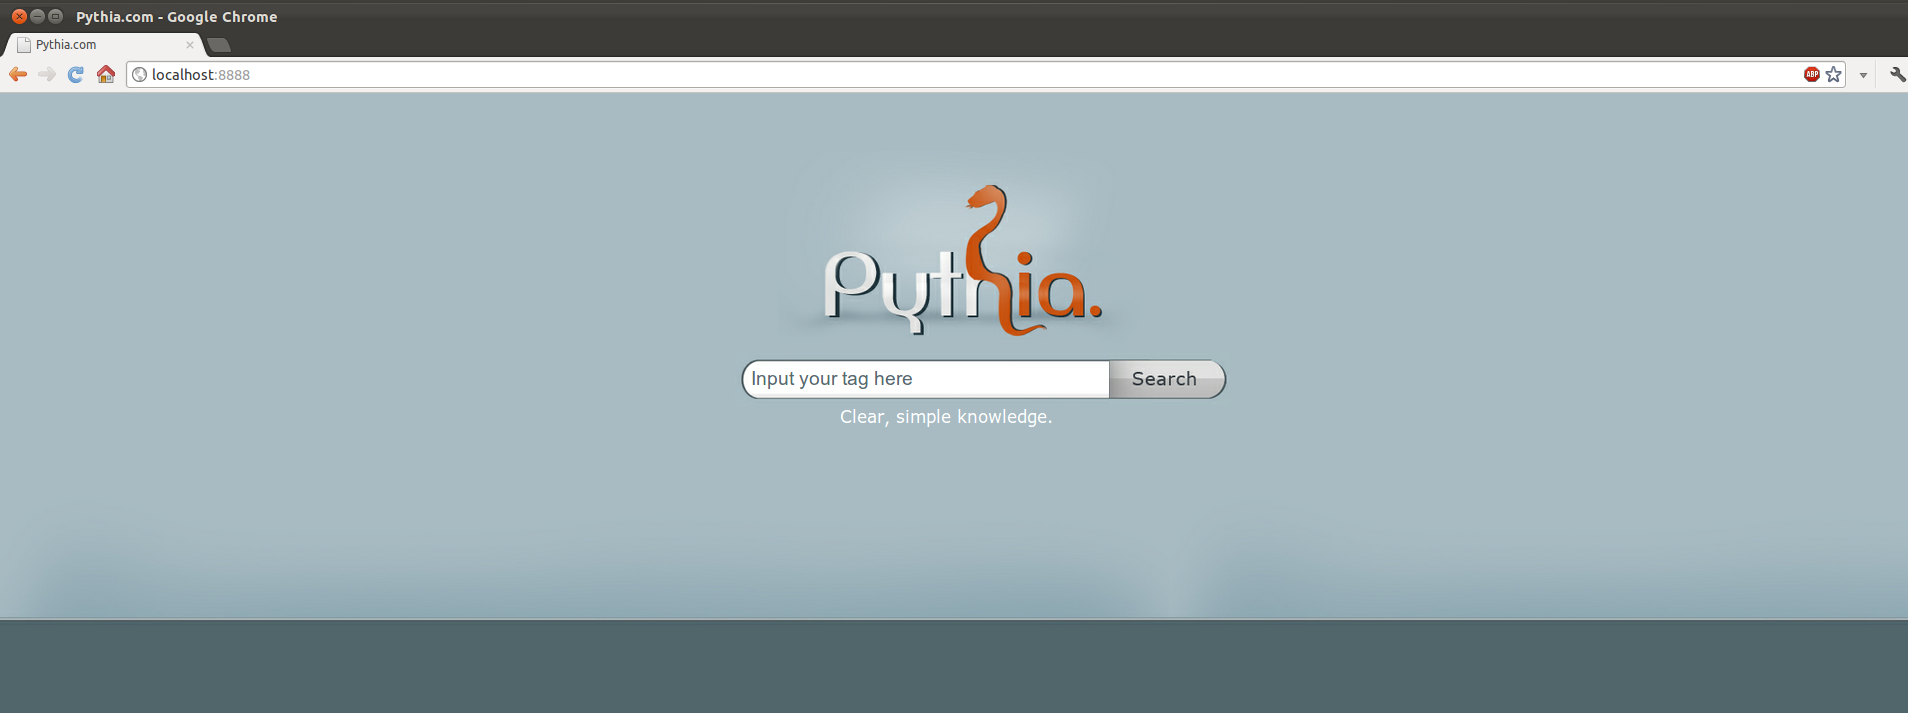
\includegraphics[height=3in, width=6in]{pythia1}
    \caption{The homepage of Pythia. The user inputs in the textbox the keywords related to the events they wish to detect.}
    \label{Pythia1}
  \end{center}
\end{figure} 
The list of keywords is send to the server and the relevan tweets are retrieved from the database. The event detection and summarisation module runs and produces the results which are send back to the user. The detected events appear as small dots on a timeline (Figure \ref{Pythia2}). The x-axis represents time and the y-axis the volume of the tweets in the dataset at that point in time. The smaller timeline on the bottom of the page is a replica of the big one and allows the user to specify a specific time period to zoom in. The timeline allows the user to see the general trend of the events and when they have occured.\\\\    
\begin{figure}[htbp]
  \begin{center}
    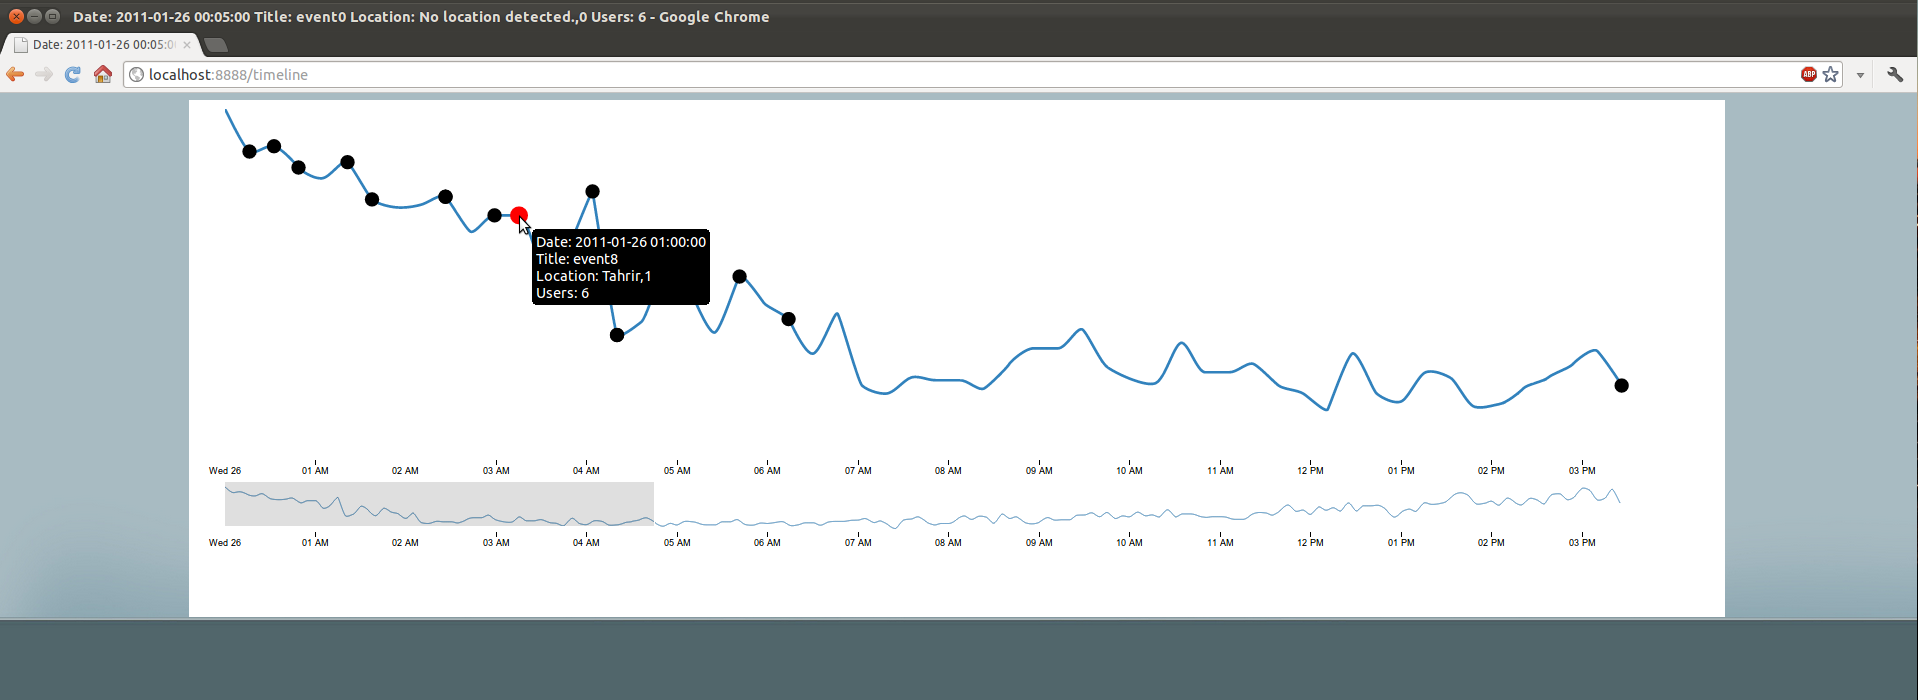
\includegraphics[height=3in, width=6in]{pythia2}
    \caption{The results are presented to the user in the form of an annotated timeline. Each dot on the timeline corresponds to a detected event. The smaller timeline at the bottom of the page allows the    user to zoom in to specific time periods.}
    \label{Pythia2}
  \end{center}
\end{figure} 
In order to understand the events more information is needed. Therefore, we have created a special popup window which displays the results of the summarisation algorithm in a human readable way. This popup window is shown in Figure \ref{Pythia3}. The user can clearly see which tweets have the highest ranking according to the LexRank algorithm and the top keywords related to the event. Additionally, if any named-entities or locations have been identified they are displayed in the relevant sections. Finally, the pie chart in the right hand corner demonstrates the results of the user classification module by showing the proportions of the user types occuring in this event.    
\begin{figure}[htbp]
  \begin{center}
    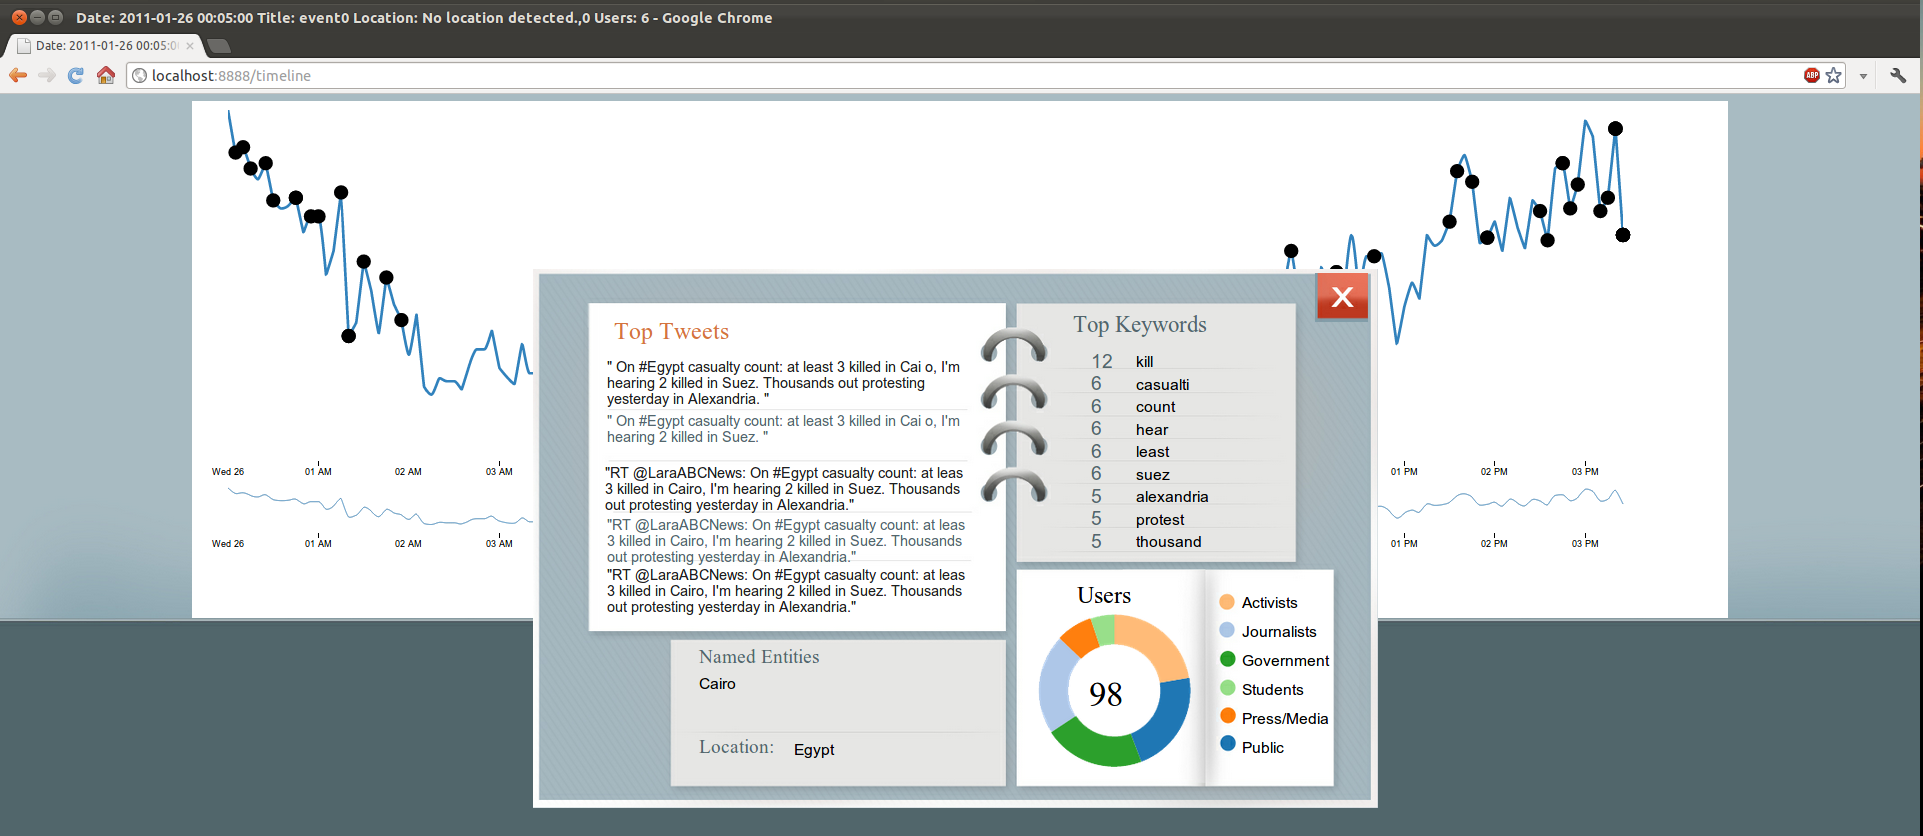
\includegraphics[height=3in, width=6in]{pythia3}
    \caption{The event summary popup helps the user understand what an event is about.}
    \label{Pythia3}
  \end{center}
\end{figure} 

\section{Case study on a clean dataset}
\subsection{Results and discussion}

\section{Case study on a real dataset}
\subsection{Results and discussion}

\section{Summary}

% ------------------------------------------------------------------------


%%% Local Variables: 
%%% mode: latex
%%% TeX-master: "../thesis"
%%% End: 

\def\baselinestretch{1}
\chapter{Conclusions}
\ifpdf
    \graphicspath{{Conclusions/ConclusionsFigs/PNG/}{Conclusions/ConclusionsFigs/PDF/}{Conclusions/ConclusionsFigs/}}
\else
    \graphicspath{{Conclusions/ConclusionsFigs/EPS/}{Conclusions/ConclusionsFigs/}}
\fi

\def\baselinestretch{1.66}

In this chapter we conclude our work by summarising our contributions and achievements in this project. We also comment on the general outcome 
of the project and based on this analysis we propose some points to be considered in potential future work in this area.\\\\
The main objective of this project was to investigate the feasibility of automatic event detection based on Twitter data. In order to 
familiarise ourselves with event detection and summarisation on Twitter we have looked at the state-of-the-art methodologies proposed by other researchers.
This background research led to the definition of three major problems that we needed to solve in our project. More specifically, these problems were
event detection, event summarisation and user classification. Event detection is achieved through clustering followed by a filtering process to remove clusters
unrelated to real world events. The remaining clusters are considered to be events and we move to the solution of the event summarisation problem. An event summary consists 
of three elements: a list of top tweets describing the event, the top keyowords of the event and the named entities occurring in the event. Two extractive summarisation
algorithms, centroid-based summarisation and LexRank are used to surface the best tweets in terms of quality, relevance and usefulness. The other two components of the summary are retrieved
using keyword weighting and named-entity recognition functions. The solution for the user classification problem is provided by machine learning classification techniques, namely decision trees and k-Nearest neighbours.\\\\
In the project achievements we also add the evaluation of the clustering and classification algorithms. Since the core component of our methodology is clustering we have focused our efforts 
on evaluating how well our algorithms perform under some circumstances which occur in Twitter datasets. The results of our evaluation helped us select the best algorithms to use
in our proof-of-concept web application, called Pythia. Pythia provides an easy to use graphical user interface enabling users to retrieve Twitter datasets and explore them. Our data mining 
toolset is the backbone of Pythia and in conjunction with the data visualisations they provide an easy to use tool for event detection and summarisation.\\\\
Reflecting back on our work we believe that the results are very promising but at the same time indicate that there is room for improvement. In particular, we believe that the strong points of our methodology are:
\begin{itemize}
  \item Using Pythia on a number of differerent datasets we have proved that is indeed possible to sift through the noise in Twitter data and extract events. This claim is supported by the evaluation results which showed that k-Means and DBSCAN with cosine similarity can cluster tweets very accurately.
  \item Event summaries were successfuly extracted since it was relatively easy for a human to identify the topic of an event by just looking at them. More specifically, the most informative part of the summaries were the top tweets since they conveyed a lot of information and almost always described the cluster's topic accurately. 
  \item If closer scrutiny of the events in needed our work showed that it is possible to classify users and investigate events pertaining to a specific type of user with relatively high accuracy.
\end{itemize}\vspace{15pt}
However, during evaluation and especially during our experience with Pythia we have identified several key problems that can be the subject of future improvements and research. We outline these problems in the next section. 

\section{Future work}

\begin{itemize}
  \item \textbf{Online clustering:} Eventhough, the performance of the online clusterer in terms of the F metric was not impressive, we believe that future work should focus on improving this algorithm. The main reason is because this algorithm can scale very easily due to its constant complexity. An improved version of the online clustering algorithm will allow us to solve completely the problem of the vast amount of tweets for an event. Additionally, our work so far focused on historical datasets meaning that users can extract events after they have actually happened. However, one might wish to detect events in real-time. This is not possible with the current implementation but a potential improved version of an online clustering algorithm can steer us towards that direction.    
  \item \textbf{Identifying real world events:} One of the first things that become apparent by using Pythia on real noisy datasets is that some detected events are not in reality real world events. The problem is the module responsible to filter our irrelevant clusters. At the moment some heuristics are used to filter out some clusters but several improvements are possible. One possible refinement is to use an automatic classifier to distinguish between event and non-event clusters. The heuristics that we use in the current implementation can be the attributes of the feature vector. The classifer will be given examples of event and non-event vectors and the classification will be automatic and probably more precise. Additionaly, more research should be conducted regarding the characteristics of real world events on Twitter in order to identify the best features to use in the classification.   
  \item \textbf{Run time performance:} We have put a lot of effort in optimising our code but there are still several bottlonecks in the implementation. Intensive vector operations such as the Euclidean distance calculation consume a large piece of the execution time and they limit the scalability of our methods. We have used several optimisation techniques and our last resort was Cython which is used to write C extensions for Python and the result is faster code. However, in future work we should investigate how the intrinsic properties of the algorithms can be optimised without the need to resort to programming solutions.     
  \item \textbf{Make use of the classification module:} We have implemented the user classification module and used it in our popup window for the summary in Pythia. It shows the distribution of different type of users in the event. However, due to time limitations we have not used the classification module for categorising tweets in the dataset according to their author. Unfortunately, this was the main motivation behind the user classification problem. Therefore, it is essential that any future work should utilise this functionality to enable users to scrutinise the dataset more closely. 
  \item \textbf{Pythia interface:} At the moment Pythia's visualisation toolset consists of the annotated timeline and the summary popup window. It is possible to make the interface more intuitive and informative. In particular, Pythia's timeline shows the overall trend in a particular dataset and shows the events as dots. However, if there are many events it is time-consuming and tedious for the user to click on each individual dot to find out what that event is about. A better approach would be to construct a timeline, similar to Twitter's timeline, that the user can easily scroll up and down.     
\end{itemize}\vspace{15pt}

%%% ----------------------------------------------------------------------

% ------------------------------------------------------------------------

%%% Local Variables: 
%%% mode: latex
%%% TeX-master: "../thesis"
%%% End: 


\backmatter % book mode only
\appendix
\chapter{Appendix}\label{Appendix}

\section{Expected events from the clean dataset}\label{EventList}

\begin{itemize}
 \item Protests in Nahya
 \item Protests in Mansour
 \item Protests in Mohandessin 
 \item Protests breaking up in various places
 \item Protests outside television building
 \item People chanting Batil in NDP
 \item Undercover police follows protesters
 \item Two protests merging
 \item Man holds up Kefaya 
 \item Protests at Maspiro building
 \item Ahramonline live coverage of the protests
 \item People leaving buses and cars to join protest
 \item Pro democracy demos have started in \#Egypt
 \item In past 8 days at least 12 people set themselves on fire out of desperation
 \item Protests in Boulak coming from Mostafa Mahmoud
 \item Early indications show numbers much larger than limited protests
 \item Amazing pictures of protesters bridge towards Opera House 
 \item Protesters are giving flowers to Policemen
 \item Al-Masry al-Youm live-streaming Egypt protests
 \item The families went down with the protesters
 \item Protests in Shubra
 \item Protests in Dar ElHekma
 \item Protesters heading towards gam3et el dowal st
 \item Protests in Alexandria 
 \item Al Jazeera Arabic is back to the news, but has nothing yet about the \#Jan25 demos
 \item Police running toward Arab League Building
 \item Protesters left Bulak and heading to Mostafa Mahmoud
 \item Guardian says: Egypt braced for a day of revolution
 \item Big demo downtown Cairo
 \item People standing at dar el qada2
 \item Incredible scenes in Ramses St - marchers breaking through police lines
 \item Demonstrations started in Dakahlia, Sharkia, Menoufia, Assiut, Kafr El Sheikh, North Sinai, Qena, Ismailia and Cairo.
 \item Thousands to Protest Against Mubarak
 \item Protesters marching past ministry of foreign affairs chanting 'Tunis'
 \item According to human rights lawyer 12 members of muslim brotherhood arrested and one journalist
 \item Protesters have taken over the nile corniche
 \item One man versus the riot police, Cairo
 \item Protesters moving back towards Supreme court. Possible circling back to Tahrir 
 
\end{itemize}\vspace{15pt}

% ------------------------------------------------------------------------

%%% Local Variables: 
%%% mode: latex
%%% TeX-master: "../thesis"
%%% End: 

\chapter{Appdx B}

and here I put some more postamble ...

% ------------------------------------------------------------------------

%%% Local Variables: 
%%% mode: latex
%%% TeX-master: "../thesis"
%%% End: 


\bibliographystyle{plainnat}
%\bibliographystyle{Classes/CUEDbiblio}
%\bibliographystyle{Classes/jmb}
%\bibliographystyle{Classes/jmb} % bibliography style
\renewcommand{\bibname}{References} % changes default name Bibliography to References
\bibliography{References/references} % References file

\end{document}
